\documentclass[12pt,a4paper]{article}
\usepackage[utf8]{inputenc}%Para Tildes y ñ%
\usepackage[spanish]{babel}
\usepackage{amsmath}
\usepackage{amsfonts}
\usepackage{amssymb}
\usepackage{adjustbox}
\usepackage{graphicx} 
\usepackage{pdfpages} %para importar paginas de un pdf 
\usepackage{booktabs}
\usepackage[bookmarks = true, colorlinks=true, linkcolor = black, citecolor = green, menucolor = black, urlcolor = black]{hyperref} 
\usepackage[left=2cm,right=2cm,top=2cm,bottom=2cm]{geometry} 
\usepackage{multirow}
\usepackage{circuitikz}
\usepackage{siunitx}
\usepackage{subfig}

\usepackage{listings}

\usepackage{verbatimbox}

\usepackage{multicol}

\usepackage{xcolor}

\usepackage{verbatimbox}
\usepackage{float}
\usepackage{textcomp}

\usepackage{caption}

\setcounter{secnumdepth}{0} % ///////////////////////////////////////////// Para que los \section no tenga numeros

\DeclareRobustCommand{\Colon}{{%
  \ooalign{%
    \hidewidth\raisebox{0.2ex}{/}\kern0.1em\hidewidth\cr
    C\cr
    \hidewidth\kern0.1em\raisebox{0.2ex}{/}\hidewidth\cr
  }%
}}

%Code listing style named "mystyle"
\lstdefinestyle{mystyle}{
  backgroundcolor=\color{backcolour}, commentstyle=\color{codegreen},
  keywordstyle=\color{magenta},
  numberstyle=\tiny\color{codegray},
  stringstyle=\color{codepurple},
  basicstyle=\ttfamily\footnotesize,
  breakatwhitespace=false,         
  breaklines=true,                 
  captionpos=b,                    
  keepspaces=true,                 
  numbers=left,                    
  numbersep=5pt,                  
  showspaces=false,                
  showstringspaces=false,
  showtabs=false,                  
  tabsize=2
}

\input{vspm.hd}

\newcommand{\keywords}[1]{\par\addvspace\baselineskip
\noindent\keywordname\enspace\ignorespaces#1}
\addto\captionsspanish{\renewcommand{\listtablename}{Índice de tablas}}		% Cambiar nombre a lista de tablas   
\addto\captionsspanish{\renewcommand{\tablename}{Tabla}}					% Cambiar nombre a tablas

\usepackage{pdfpages}
\usepackage{enumerate}%listas y viñetas
\author{ Leonardo Serrano Arias C17484  \\Lorena Solís Extteny B97657\\{\small }\\ \\ Profesor: Marco Villalta  \vspace*{3.0in}}
\title{Universidad de Costa Rica\\{\small Facultad de Ingeniería\\Escuela de Ingeniería Eléctrica\\IE0624 – Laboratorio de Microcontroladores\\II ciclo 2024\\\vspace*{0.55in} Laboratorio \# 4 }\\ STM32: GPIO, ADC, comunicaciones, Iot \vspace*{1.35in}}
\date{30 de Octubre, 2024} 

\lstset{style=mystyle}
\begin{document} 

\maketitle  
\thispagestyle{empty}%%no numerar la portada
\renewcommand{\thepage}{\roman{page}}
\newpage
\tableofcontents

\listoffigures 

%\listoftables  

%%%%%%%%%%  
\renewcommand{\thepage}{\arabic{page}} 
\setcounter{page}{1}

\newpage
\section{Introducción}
Este informe detalla el diseño y desarrollo de un sismógrafo digital, implementado con la placa STM32F429 Discovery Kit y la biblioteca libopencm3. El dispositivo está alimentado por una batería y se utiliza para registrar y analizar oscilaciones en el entorno. Entre las funcionalidades incluidas están la lectura de los ejes del giroscopio, el monitoreo del nivel de batería, y la habilitación de comunicación mediante USART/USB. Para facilitar el monitoreo remoto, se implementa una conexión con la plataforma IoT Thingsboard, permitiendo la visualización de las mediciones y el estado del dispositivo a distancia.
El repositorio utilizado para el desarrollo de este laboratorio se encuentra en la siguiente dirección: \url{https://github.com/Leonardo-SA/IE-0624_II_2024_C17484_B97657.git}

\section{Nota teórica}

\subsection{STM:32F429}
El STM32F429 \cite{hoja}es un microcontrolador de la serie STM32 de STMicroelectronics, caracterizado por su alta capacidad de procesamiento y múltiples interfaces de comunicación, lo que lo convierte en una opción ideal para aplicaciones avanzadas. El STM32F429 cuenta con una Unidad de Punto Flotante (FPU) y una amplia gama de periféricos, como ADC (Convertidores Analógico-Digitales) y USART (Transmisor-Receptor Asíncrono Universal). Estas características permiten realizar cálculos complejos y gestionar comunicaciones de manera eficiente, lo cual es fundamental para el funcionamiento de un sismógrafo digital que requiere un procesamiento rápido de los datos del giroscopio y un monitoreo constante del nivel de batería.

A continuación se muestra el diagrama de pines:

\begin{figure}[H]
    \centering
    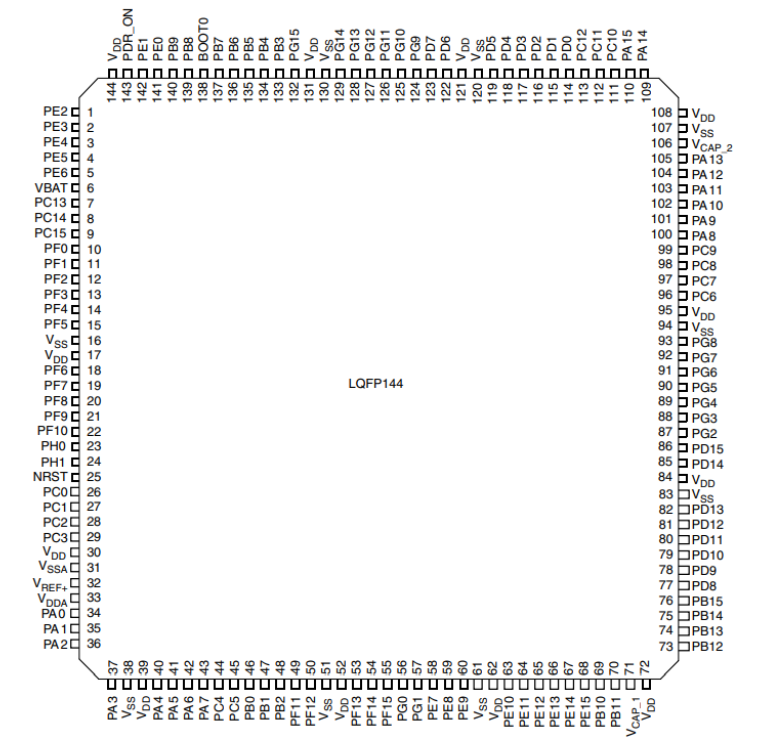
\includegraphics[width=0.7\linewidth]{Imagenes/pins.png}
    \caption{Diagrama de pines del STM32F429 \cite{hoja}}
    \label{fig:1}
\end{figure}

En la siguiente figura es posible apreciar el diagrama de bloques de este microcontrolador:

\begin{figure}[H]
    \centering
    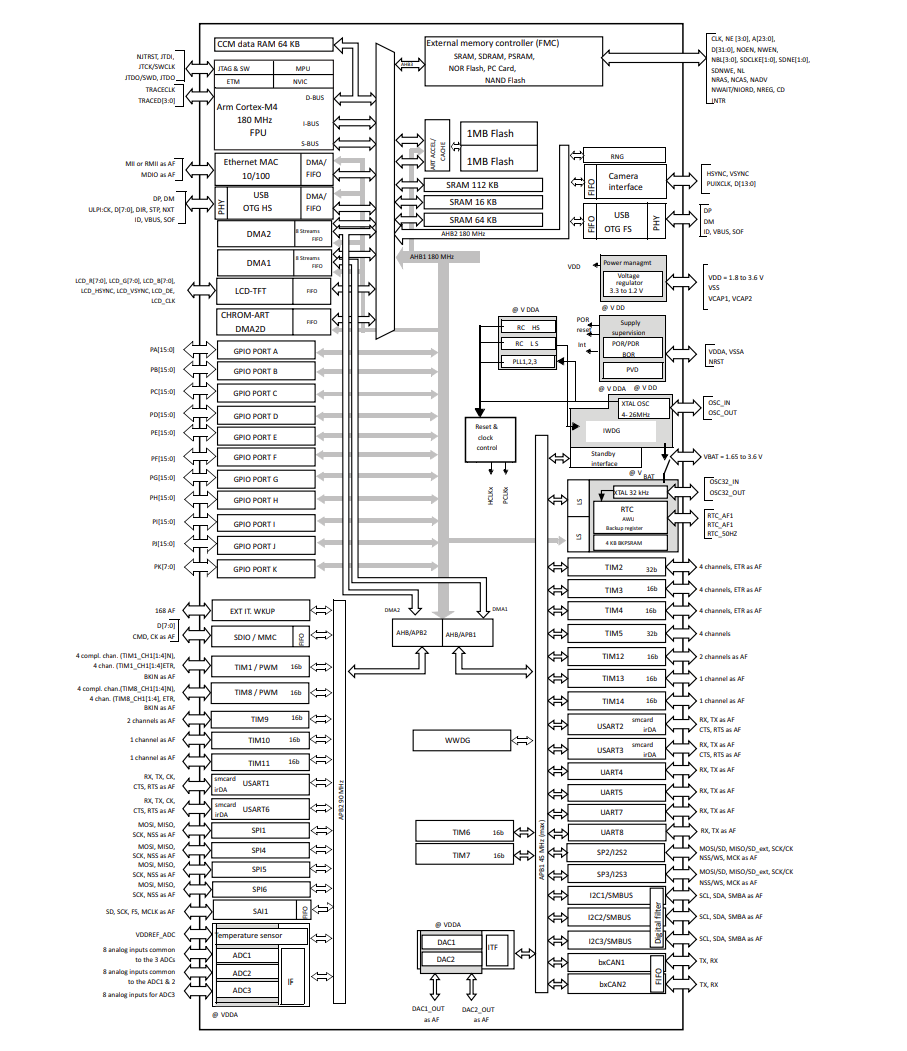
\includegraphics[width=0.9\linewidth]{Imagenes/block.png}
    \caption{Diagrama de bloques del STM32F429 \cite{hoja}}
    \label{fig:1}
\end{figure}

Algunas características de este microcontrolador se menncionan a continuación \cite{hoja}:

\begin{itemize}
    \item Microcontrolador STM32F429ZI con 2 Mbytes de memoria Flash, 256 Kbytes de RAM en un encapsulado LQFP144.
    \item ST-LINK/V2 integrado en 32F429IDISCOVERY o ST-LINK/V2-B en STM32F429I-DISC1.
    \item Soporte para ARM\textsuperscript{\textregistered} mbed\textsuperscript{TM} (http://mbed.org) con ST-LINK/V2-B solamente.
    \item ST-LINK USB con capacidad de re-enumeración y tres interfaces diferentes:
    \begin{itemize}
        \item Puerto COM virtual (solo con ST-LINK/V2-B).
        \item Almacenamiento masivo (solo con ST-LINK/V2-B).
        \item Puerto de depuración.
    \end{itemize}
    \item Alimentación de la placa: a través del bus USB o mediante una fuente externa de 3 V o 5 V.
    \item Pantalla TFT LCD QVGA de 2.4".
    \item SDRAM de 64 Mbits.
    \item Sensor de movimiento L3GD20, giroscopio digital de tres ejes con salida digital.
    \item Seis LEDs:
    \begin{itemize}
        \item LD1 (rojo/verde) para comunicación USB.
        \item LD2 (rojo) para indicador de encendido de 3.3 V.
        \item Dos LEDs de usuario: LD3 (verde), LD4 (rojo).
        \item Dos LEDs OTG USB: LD5 (verde) para VBUS y LD6 (rojo) para OC (sobrecorriente).
    \end{itemize}
    \item Dos botones pulsadores (usuario y reset).
    \item Conector USB OTG con conector micro-AB.
    \item Conector de expansión para LQFP144 I/Os, que permite una conexión rápida a la placa de prototipos y facilita el sondeo.
    \item Software libre completo que incluye una variedad de ejemplos, como parte de STM32CubeF4 package o STSW-STM32138 para uso con bibliotecas estándar heredadas.
\end{itemize}

En cuanto a las características eléctricas las siguientes tablas presentan la información de voltajes y corrientes:

\begin{table}[h!]
\centering
\caption{Características de voltaje \cite{hoja}}
\resizebox{\textwidth}{!}{%
\begin{tabular}{|>{\centering\arraybackslash}m{3cm}|>{\centering\arraybackslash}m{8cm}|>{\centering\arraybackslash}m{2cm}|>{\centering\arraybackslash}m{2cm}|>{\centering\arraybackslash}m{2cm}|}
\hline
\textbf{Símbolo} & \textbf{Especificaciones} & \textbf{Mín} & \textbf{Máx} & \textbf{Unidad} \\
\hline
$V_{DD}-V_{SS}$ & Voltaje principal de alimentación externo (incluye $V_{DDA}$, $V_{DD}$ y $V_{BAT}$)\textsuperscript{(1)} & -0.3 & 4.0 & V \\
\hline
$V_{IN}$ & Voltaje de entrada en pines FT\textsuperscript{(2)} & $V_{SS}-0.3$ & $V_{DD}+4.0$ & V \\
\hline
$V_{IN}$ & Voltaje de entrada en pines TTa & $V_{SS}-0.3$ & 4.0 & V \\
\hline
$V_{IN}$ & Voltaje de entrada en cualquier otro pin & $V_{SS}-0.3$ & 4.0 & V \\
\hline
$V_{IN}$ & Voltaje de entrada en el pin BOOT0 & $V_{SS}$ & 9.0 & V \\
\hline
$\left| \Delta V_{DDx} \right|$ & Variaciones entre diferentes pines de alimentación $V_{DD}$ & - & 50 & mV \\
\hline
$\left| V_{SSX}-V_{SS} \right|$ & Variaciones entre todos los pines de tierra incluyendo $V_{REF-}$ & - & 50 & mV \\
\hline
$V_{ESD(\text{HBM})}$ & Voltaje de descarga electrostática (modelo de cuerpo humano) & \multicolumn{3}{c|}{} \\
\hline
\end{tabular}%
}
\end{table}



\begin{table}[h!]
\centering
\caption{Características de corriente \cite{hoja}}
\resizebox{\textwidth}{!}{%
\begin{tabular}{|>{\centering\arraybackslash}m{3cm}|>{\centering\arraybackslash}m{8cm}|>{\centering\arraybackslash}m{2cm}|>{\centering\arraybackslash}m{2cm}|}
\hline
\textbf{Símbolo} & \textbf{Especificaciones} & \textbf{Máx.} & \textbf{Unidad} \\
\hline
$\sum I_{VDD}$ & Corriente total de entrada en todas las líneas de alimentación $V_{DD_x}$ (fuente)\textsuperscript{(1)} & 270 & mA \\
\hline
$\sum I_{VSS}$ & Corriente total de salida en todas las líneas de tierra $V_{SS_x}$ (sumidero)\textsuperscript{(1)} & -270 & mA \\
\hline
$I_{VDD}$ & Corriente máxima de entrada en cada línea de alimentación $V_{DD_x}$ (fuente)\textsuperscript{(1)} & 100 & mA \\
\hline
$I_{VSS}$ & Corriente máxima de salida en cada línea de tierra $V_{SS_x}$ (sumidero)\textsuperscript{(1)} & -100 & mA \\
\hline
$I_{IO}$ & Corriente de salida hundida por cualquier pin de I/O o de control & 25 & mA \\
\hline
$I_{IO}$  & Corriente de salida suministrada por cualquier pin de I/O o de control & -25 & mA \\
\hline
$\sum I_{IO}$ & Corriente total de salida hundida por todos los pines de I/O y de control\textsuperscript{(2)} & 120 & mA \\
\hline
$\sum I_{IO}$  & Corriente total de salida suministrada por todos los pines de I/O y de control\textsuperscript{(2)} & -120 & mA \\
\hline
$I_{INJ(PIN)}$ & Corriente inyectada en pines FT\textsuperscript{(4)} & -5/+0 & mA \\
\hline
$I_{INJ(PIN)}$  & Corriente inyectada en los pines NRST y BOOT0\textsuperscript{(4)} & -5/+0 & mA \\
\hline
$I_{INJ(PIN)}$  & Corriente inyectada en pines TTa\textsuperscript{(5)} & $\pm$5 & mA \\
\hline
$\sum I_{INJ(PIN)}$ & Corriente total inyectada en todos los pines de I/O y de control\textsuperscript{(6)} & $\pm$25 & mA \\
\hline
\end{tabular}%
}
\end{table}

\subsection{Sensor L3GD20}
El L3GD20\cite{sensor} es un giroscopio de tres ejes utilizado en este proyecto para detectar las variaciones en las oscilaciones en los ejes X, Y y Z. Este sensor de movimiento permite capturar cambios en la orientación y velocidad angular, facilitando así la detección precisa de movimientos del edificio. Sus datos son críticos para registrar las oscilaciones y movimientos que pueden ser causados por vibraciones estructurales, ya que estos valores serán transmitidos al sistema IoT. Seguidamente, se muestra el diagrama de pines del mismo:
\begin{figure}[H]
    \centering
    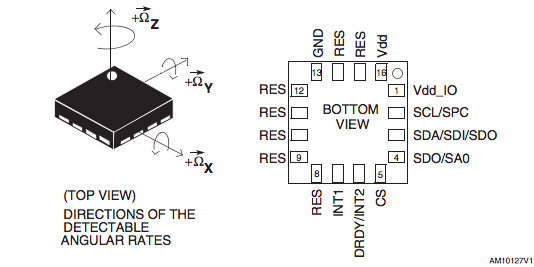
\includegraphics[width=0.9\linewidth]{Imagenes/sensor.png}
    \caption{Diagrama de pines del sensor L3GD20\cite{sensor}}
    \label{fig:1}
\end{figure}

\subsection{Pantalla LCD/TFT ILI9341}
La pantalla  LCD/TFT ILI9341 \cite{hoja} es una pantalla táctil a color que permite la visualización de datos en una resolución de 240x320 píxeles. Además, esta cuenta con un controlador gráfico(\textbf{ILI9341}) que facilita la gestión y representación de gráficos en la misma. También cuenta con un controlador táctil (\textbf{XPT2046}) que hace posible la interación táctil. Finalmente, utiliza comunicaciones I2C/SPI que se conecta en el Discovery Kit a través del bus SPI5.

\subsection{GPIOs (General Purpose Input/Output)}

Los pines GPIO del STM32F429 \cite{gpio} permiten conectar y configurar dispositivos externos en modos de entrada, salida, función alternativa o analógico. En este laboratorio, se plantea utilizar el pin PB0 para configurar en modo analógico las lecturas del voltaje de la batería a través del canal ADC1 IN8, lo cual permitiría el monitoreo continuo del nivel de carga.

\subsection{ADC}
El ADC es un componente que permite la conversión de señales analógicas en digitales. En el caso de este laboratorio, el ADC se desea emplear para medir el nivel de voltaje de la batería. Con una lectura continua del voltaje, es posible determinar el nivel de carga restante y activar una alerta en caso de que el nivel esté cerca del mínimo requerido para el funcionamiento seguro del sistema, asegurando así una operación estable y segura del sismógrafo. \cite{hoja}

\subsection{Comunicaciones}
La implementación del sismógrafo digital se apoya en diferentes protocolos de comunicación, cada uno con una función específica en el sistema. A continuación, se describe el uso de cada protocolo:

\subsubsection{USART}
 El protocolo USART \cite{usart} es fundamental en este laboratorio para la comunicación serie asíncrona entre el microcontrolador y otros dispositivos externos. Este protocolo permite la transmisión y recepción de datos sin requerir un reloj compartido, lo cual es ventajoso para comunicaciones de bajo costo y configuraciones de largo alcance. En el caso del sismógrafo, UART es utilizado para enviar datos críticos como los valores del giroscopio en los ejes X, Y y Z, y el nivel de batería. Estos datos son recibidos por un script en Python que los envía a un dashboard IoT para la visualización remota y en tiempo real del estado del sistema. 

\subsubsection{SPI}
La interfaz SPI \cite{spi} es un protocolo de comunicación sincrónico ideal para la transferencia rápida de datos entre el microcontrolador y otros periféricos. En este laboratorio, SPI se utiliza para la comunicación con el display LCD y el sensor de movimiento L3GD20. SPI permite una transmisión de datos más rápida en comparación con UART, lo cual es especialmente útil para la actualización de imágenes en la pantalla y la lectura continua de datos del giroscopio. La comunicación SPI se basa en un modelo maestro-esclavo, donde el STM32F429 actúa como maestro controlando el reloj y la sincronización de los datos enviados y recibidos. 

\subsubsection{USB}
El USB \cite{usb} es una interfaz de comunicación versátil utilizada para la transmisión de datos y la depuración del sistema. Además de soportar modos de depuración y emulación de puerto serie, el USB también ofrece funciones de almacenamiento masivo, permitiendo al dispositivo actuar como una unidad de almacenamiento externa cuando está conectado a una computadora. Esto facilita la transferencia de archivos y la actualización de firmware. La placa STM32F429 Discovery también puede alimentarse a través del puerto USB o mediante una fuente externa de 3V o 5V, lo que otorga flexibilidad en las opciones de alimentación y asegura que el dispositivo continúe operando incluso si el suministro principal es interrumpido. 

\subsection{IoT (Internet of Things)}
El Internet de las Cosas (IoT) se refiere a la interconexión de dispositivos y sistemas a través de la red. El sismógrafo digital envía datos a la plataforma IoT Thingsboard a través de un script en Python que recibe los datos por comunicación serial desde el microcontrolador. Esto permite monitorear las mediciones y el estado del dispositivo en tiempo real desde una ubicación remota.\cite{iot}


\section{Hardware}%Diseño del circuito


\subsection{Tabla de componentes electrónicos}

A continuación, se muestra una tabla con los componentes utilizados para el desarrollo del proyecto:

\begin{table}[H]
\centering
\caption{Componentes con el precio por unidad }
\begin{tabular}{|cc|c|}
\hline
\multicolumn{1}{|c|}{\textbf{Componente}} & \textbf{Cantidad} & \textbf{Precio($\Colon$)} \\ \hline
\multicolumn{1}{|c|}{STM32F429 Discovery kit} & 1 & 15000 \\ \hline
\multicolumn{1}{|c|}{Batería 9V} & 1 & 3340 \\ \hline
\multicolumn{1}{|c|}{Broche para batería de 9V} & 1 & 250 \\ \hline
\multicolumn{1}{|c|}{Resistencia de $1000\Omega$} & 1 & 15 \\ \hline
\multicolumn{1}{|c|}{Resistencia de $220\Omega$} & 1 & 15 \\ \hline
\multicolumn{1}{|c|}{Resistencia de $330\Omega$} & 1 & 15 \\ \hline
\multicolumn{1}{|c|}{Protoboard} & 1 & 5500 \\ \hline
\multicolumn{2}{|c|}{Total} &  24135\\ \hline
\end{tabular}
\label{tab:my-table}
\end{table}

\subsection{Firmware y libopencm3}
A continuación, se describen las principales librerías utilizadas y su respectiva función:
\begin{itemize}

    \item \textbf{clock.h}:Contiene las declaraciones de funciones para la configuración y control del sistema de reloj en el microcontrolador.
    \item \textbf{console.h}:Define una serie de funciones para la configuración y operación de una consola a través de un puerto serie utilizando el periférico USART.
    \item \textbf{sdram.h}:Define la interfaz para la inicialización y el manejo de la memoria SDRAM.
    \item \textbf{lcd-spi.h}:Define la interfaz y configuración para controlar una pantalla LCD mediante el protocolo SPI.
    \item \textbf{gfx.h}:Define las funciones gráficas de propósito general para el manejo de gráficos en la pantalla TFT/LCD.
    
\end{itemize}

\subsection{Archivos de libopencm3}
Para el desarrollo del laboratorio se utilizaron archivos del repositorio de libopencm3 \cite{libopencm3} donde se tomaron scripts de los ejemplos que incluye para agilizar el la elaboración, acontinuación se explica cada uno de ellos:
\begin{itemize}
    \item \textbf{clock.c}: Este contiene las funciones para configurar los ajustes del clock.
    \item \textbf{console.c}: Este es un ring buffer que mantiene los caracteres a medida que son escritos.
    \item \textbf{gfx.c}: Se encarga de manejar la manipulación gráfica.
    \item \textbf{lcd-spi.c}: Este archivo implementa la comunicación SPI para poder interactuar con la pantalla.
    \item \textbf{sdram.c}: Permite la configuración y operación de la SDRAM, que almacena temporalmente los datos.
    \item \textbf{spi-mems.c}:Implementa la comunicación SPI que interactúa con el giroscopio MEMS.
\end{itemize}

\section{Desarrollo}

\subsection{Diagrama de flujo}
Seguidamente, se muestra el diagrama de flujo que se desarrolla para el sismógrafo:

\begin{figure}[H]
    \centering
    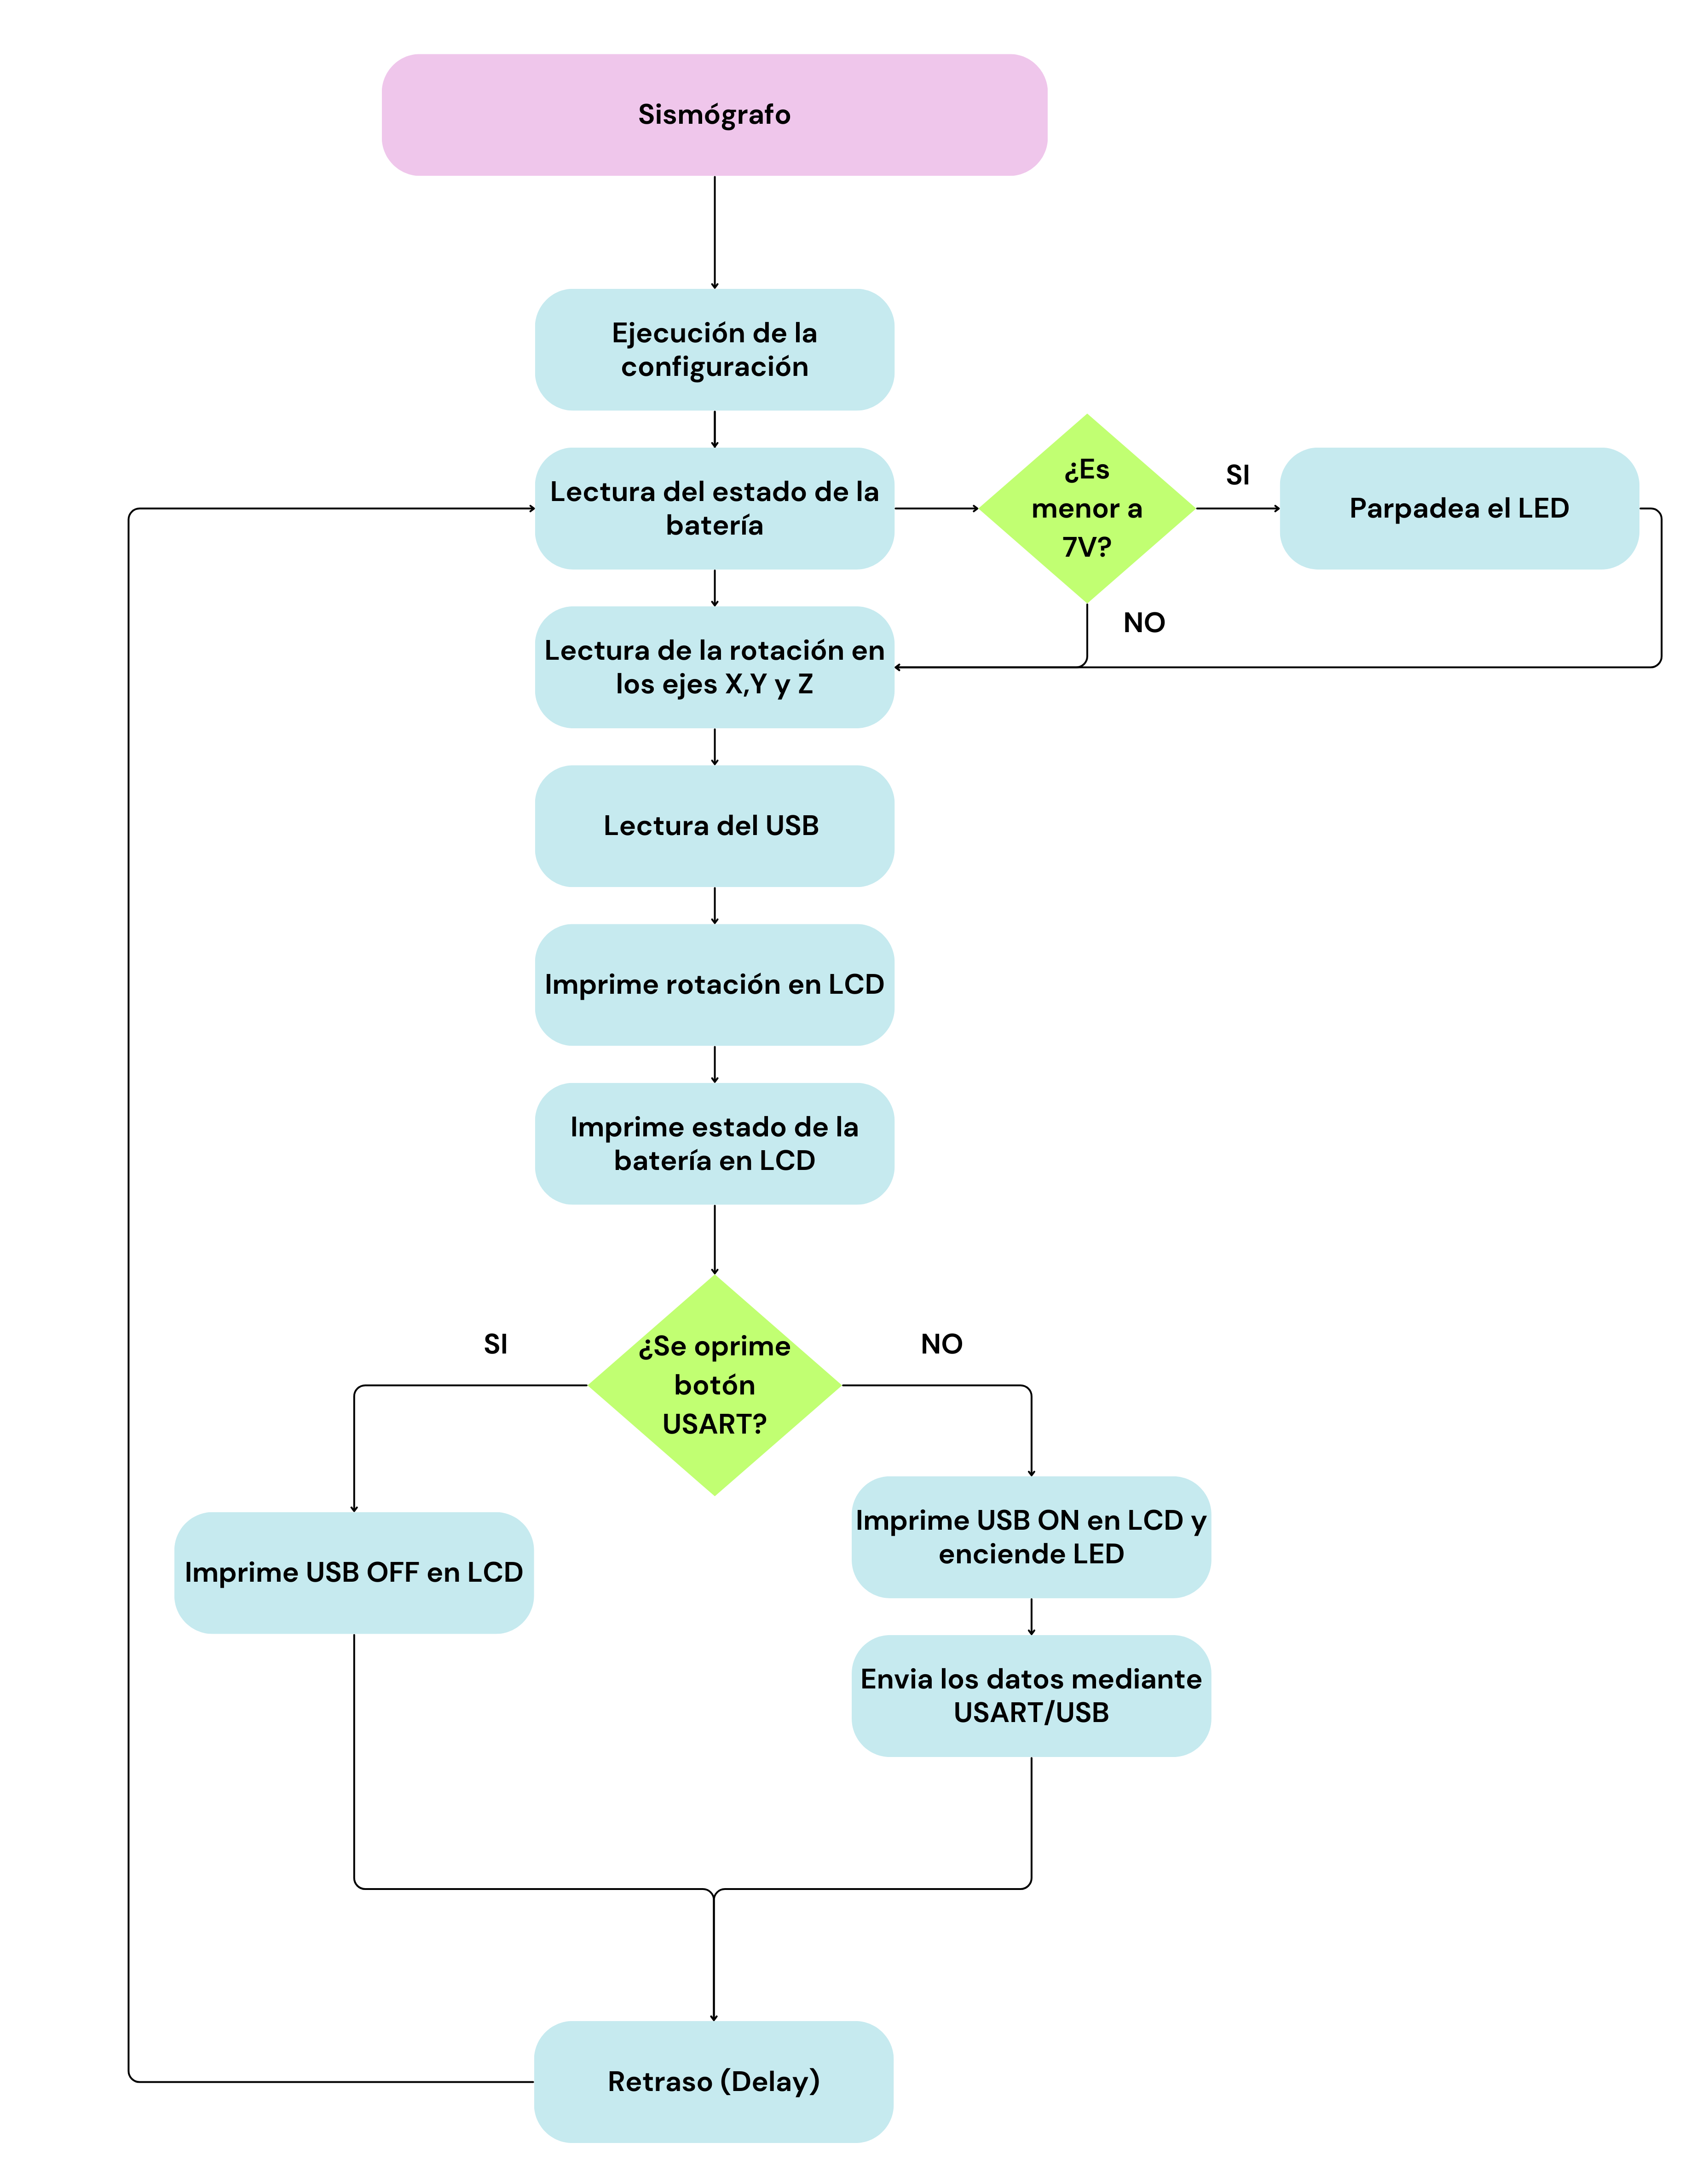
\includegraphics[width=0.5\linewidth]{Imagenes/df.png}
    \caption{Diagrama de flujo del Sismógrafo}
    \label{fig:5}
\end{figure}

\subsection{Diseño del circuito con divisor de tensión}
Para realizar el diseño del circuito es necesario desarrollar un divisor de tensión. Lo cual es fundamental para la correcta alimentación del sistema y la medición del nivel de tensión de la batería. A continuación, se realizó el calculo del divisor de tensión considerando que se tiene una resistencia de  $R_1=1000\Omega$ y otra de $R_2=550\Omega$, de manera que se obtiene lo siguiente:

\begin{equation*}
\begin{split}
    V_{out}= V{in} \cdot \frac{R_1}{R_2+R_1} \\
    V_{out}=7,55 \cdot \frac{1000\Omega}{550\Omega+1000\Omega} \\
    V_{out}= \frac{151}{31} \approx 4,87 V
\end{split}
\end{equation*}

Por lo tanto, gracias a este divisor de tensión se garantiza una segura utilización de la batería con el microcontrolador para que esta no supere los límites de tensión del mismo. 

\subsection{Funcionamiento del circuito}
Se diseñó un código capaz de recrear  un sismógrafo digital en el microcontrolador STM32F429. Para ello se debió implementar las siguentes funcionalidades:

\begin{itemize}
    \item Capturar los valores de los ejes del giroscopio (X, Y, Z).
    \item Añadir un interruptor o botón que permita activar o desactivar las comunicaciones mediante USART/USB.
    \item Implementar un LED que parpadee para indicar que la transmisión o recepción de datos mediante USART/USB está activa.
    \item Medir el nivel de carga de la batería en un rango de [0,9]V. Si la batería se aproxima al nivel mínimo operativo del microcontrolador, se debe activar un LED de alerta intermitente y enviar una notificación de batería baja al tablero de control en Thingsboard.
    \item Mostrar en la pantalla LCD el nivel de carga de la batería, los valores de los ejes X, Y y Z, y el estado de la comunicación serial/USB.
    \item Crear un script en Python que lea o escriba datos en el puerto serial/USB y que envíe la información del giroscopio y el nivel de batería a un tablero de IoT en thingsboard.
\end{itemize}

Al encender el Discovery Kit y cargar el código principal al microcontrolador se puede ver lo siguiente en la pantalla.
\begin{figure}[H]
    \centering
    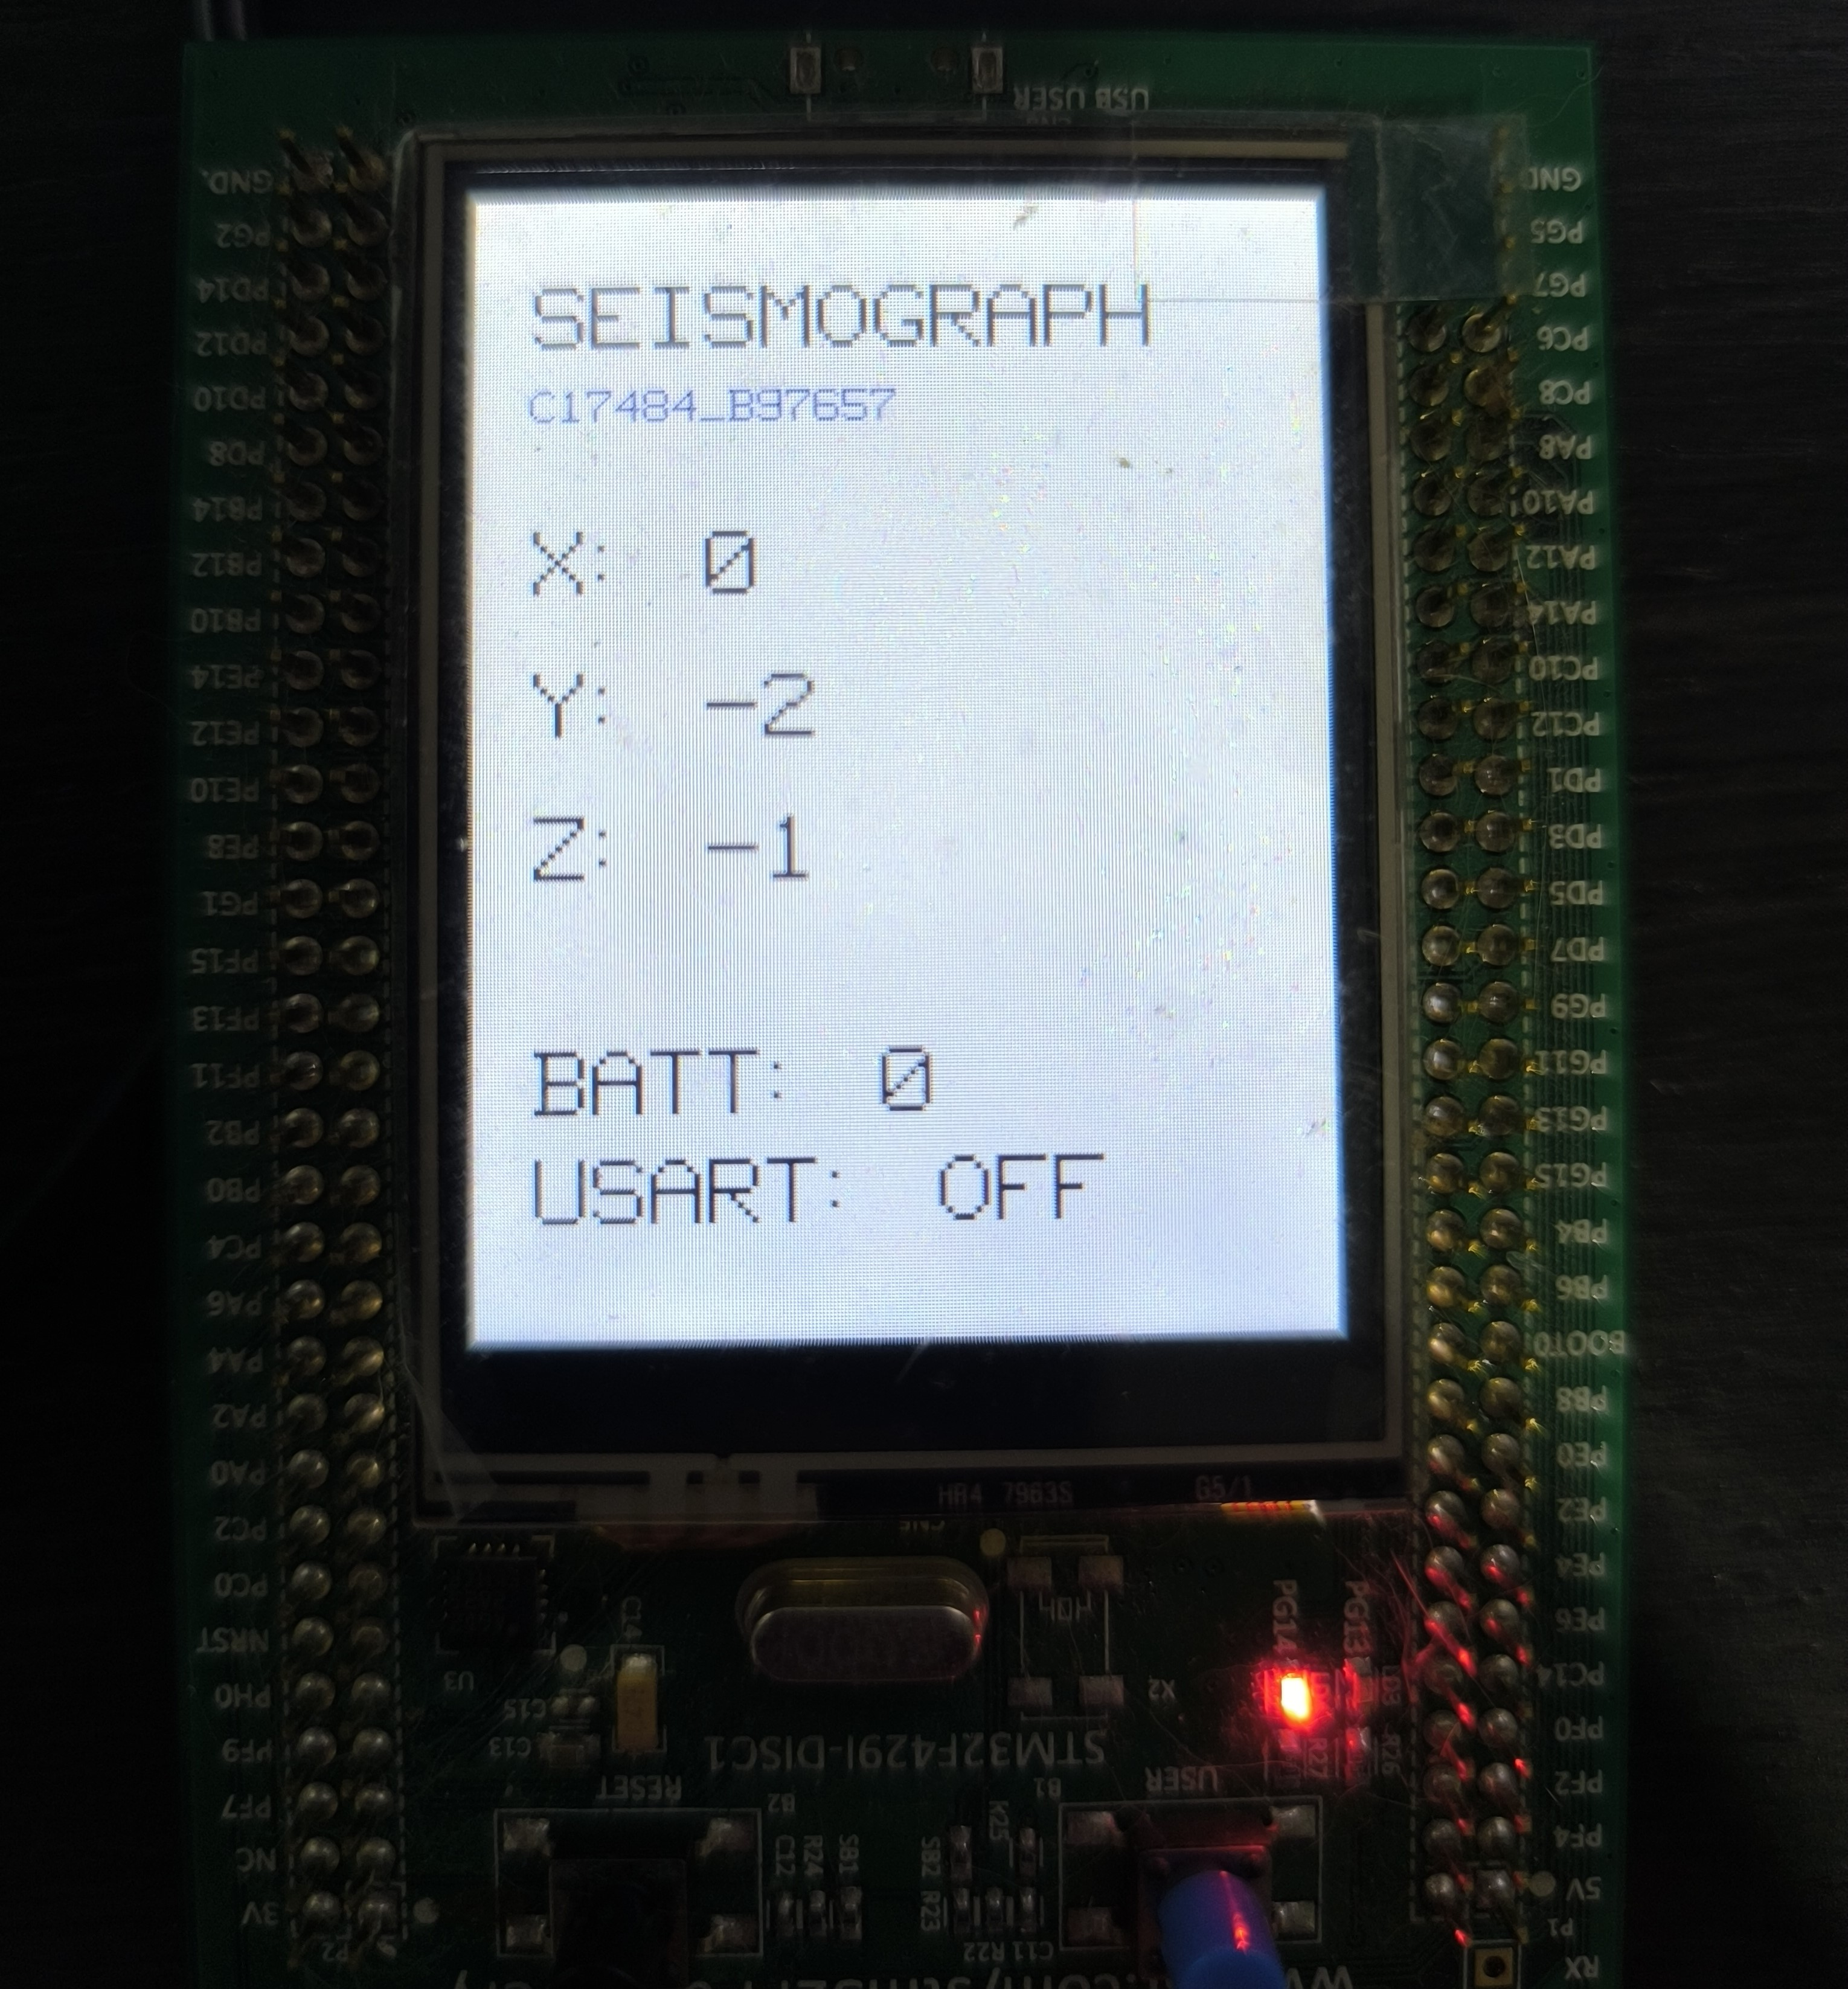
\includegraphics[width=0.5\linewidth]{Imagenes/mcu.jpg}
    \caption{STM32F429 Discovery Kit encendido}
    \label{fig:5}
\end{figure}

En esta pantalla se muestran los valores de los ejes (xyz), el nivel de batería y el estado de la comunicación USART/USB.  

Cuando se gira en alguno de los ejes el giroscopio incluido en la placa es posible notar cómo se alteran los valores en la pantalla, tal como en la siguiente imagen.

\begin{figure}[H]
    \centering
    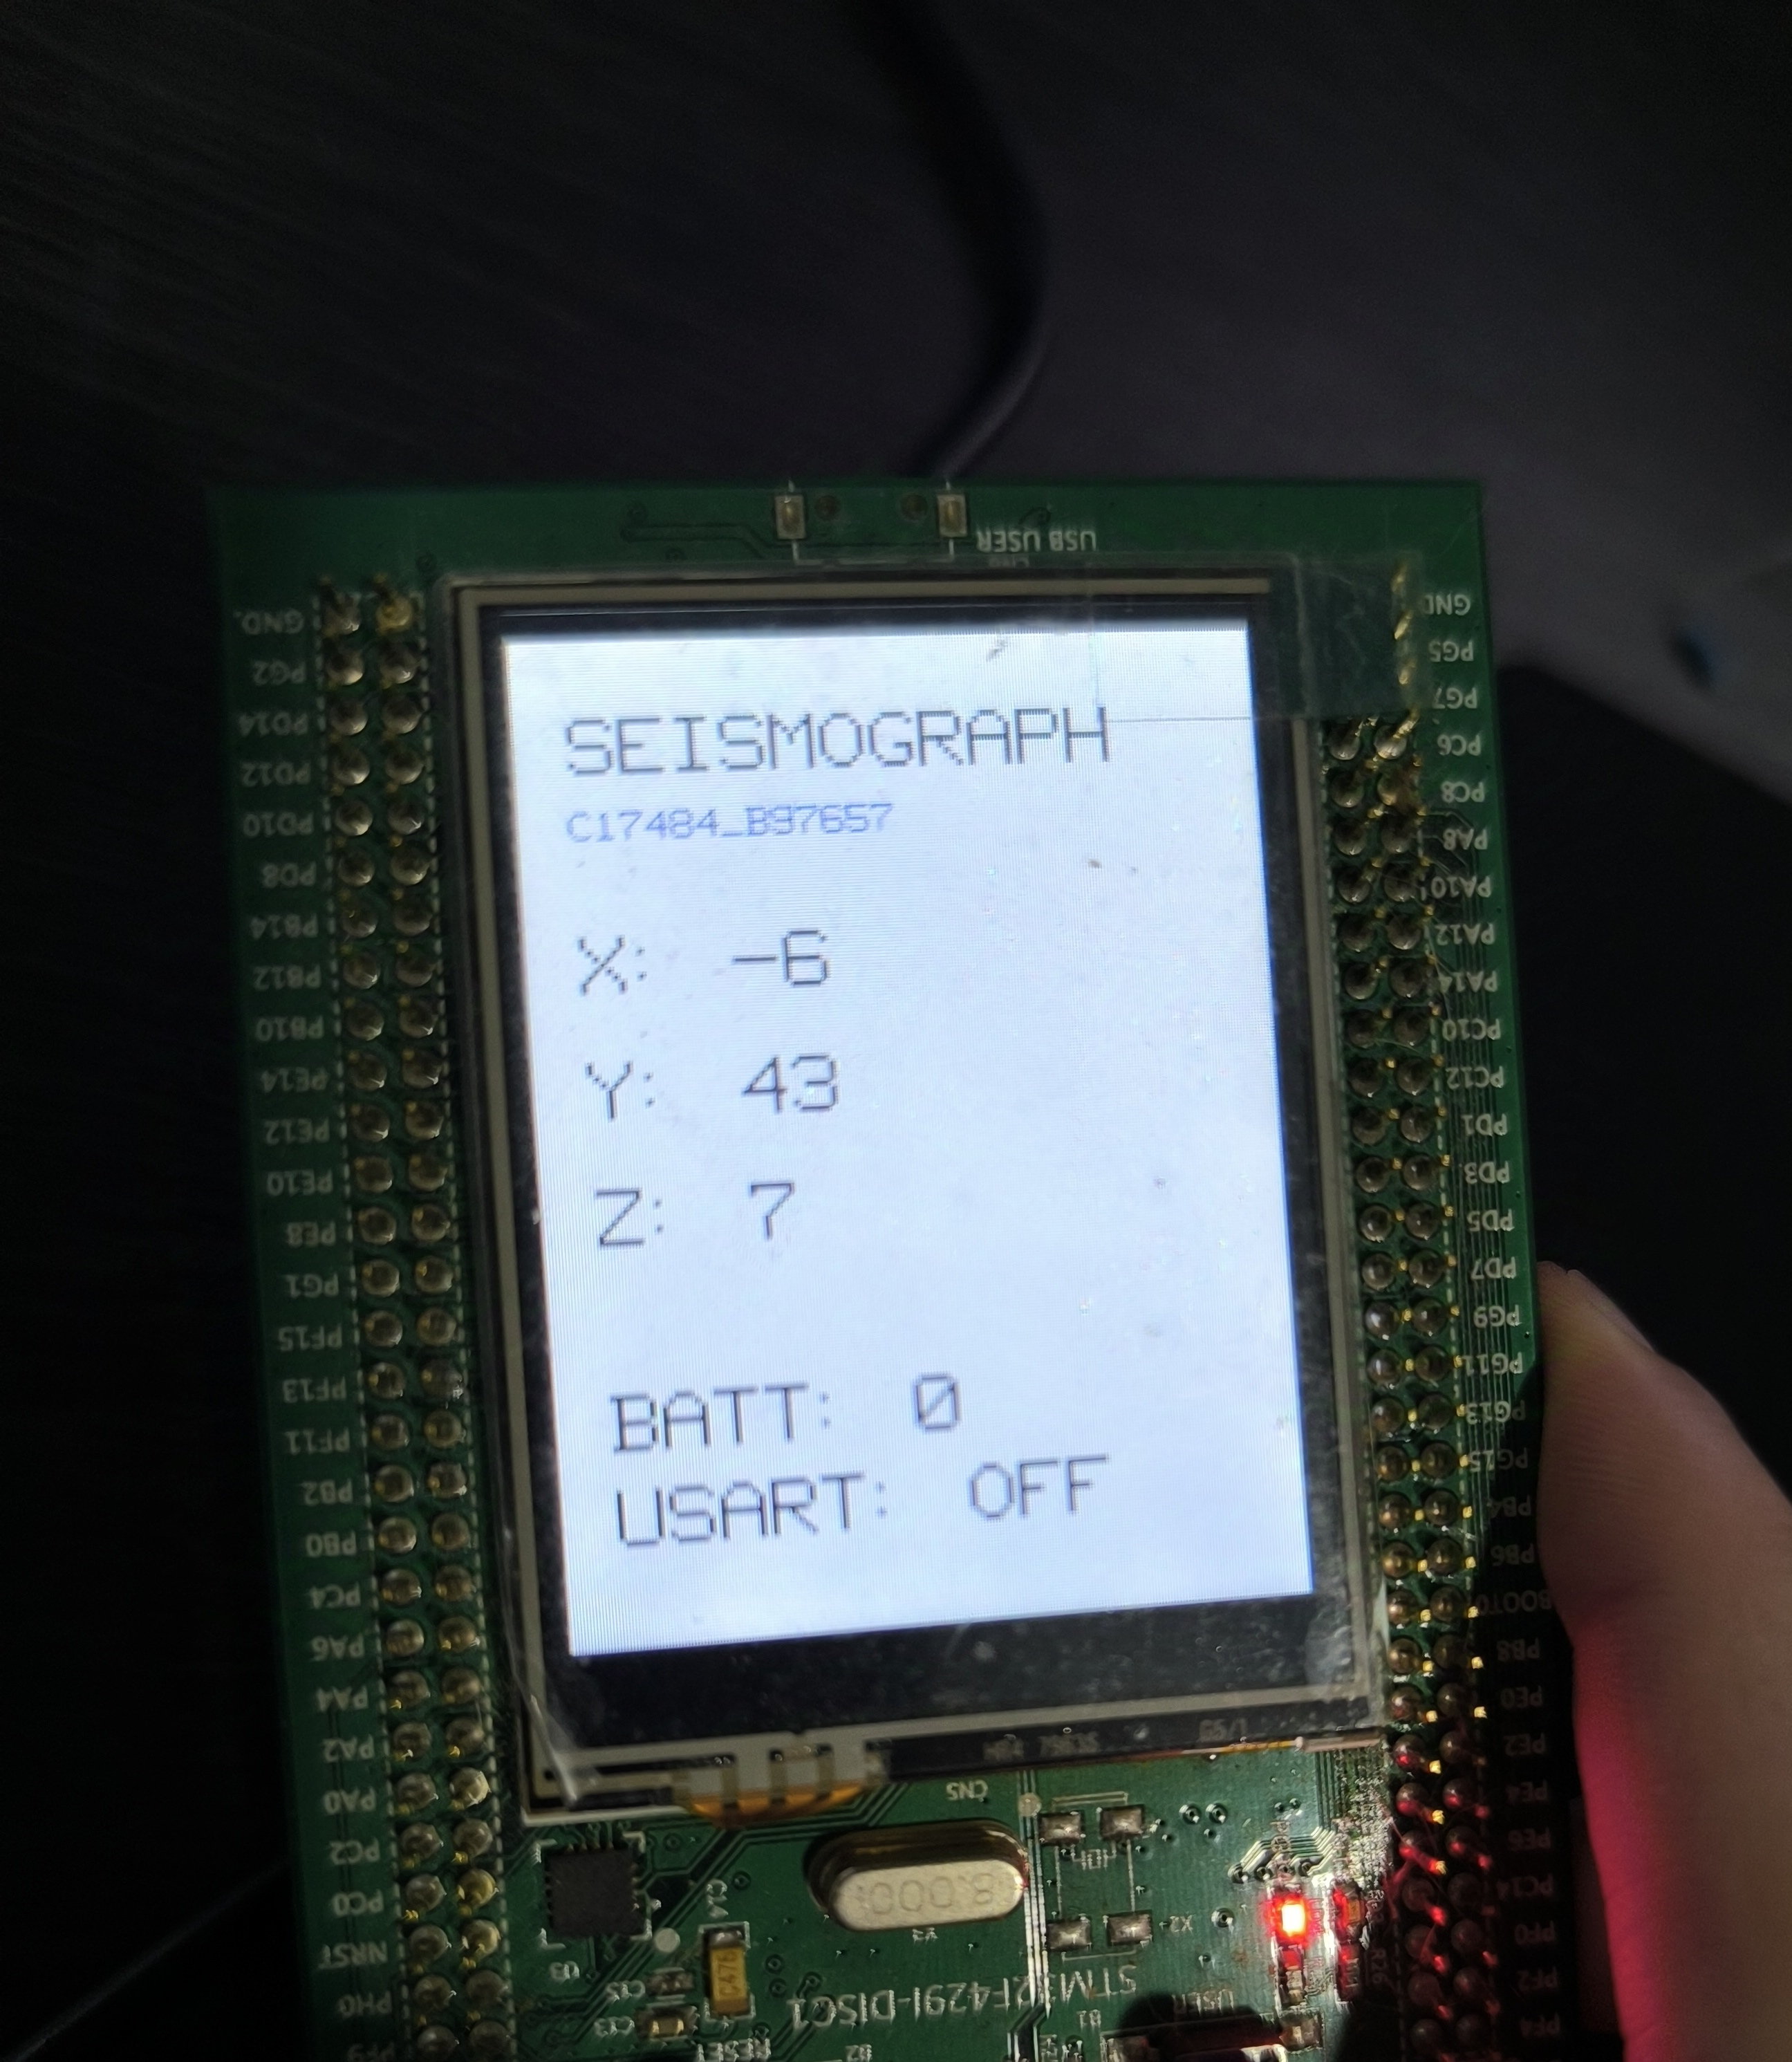
\includegraphics[width=0.5\linewidth]{Imagenes/gyr.jpg}
    \caption{Lectura de valores de los ejes del giroscopio}
    \label{fig:5}
\end{figure}

Por otro lado, el sismógrafo está conectado a una batería de 9V, con un regulador de voltaje a 5V, el cual es el suministro de voltaje externo recomendado.

El circuito se muestra a continuación:
\begin{figure}[H]
    \centering
    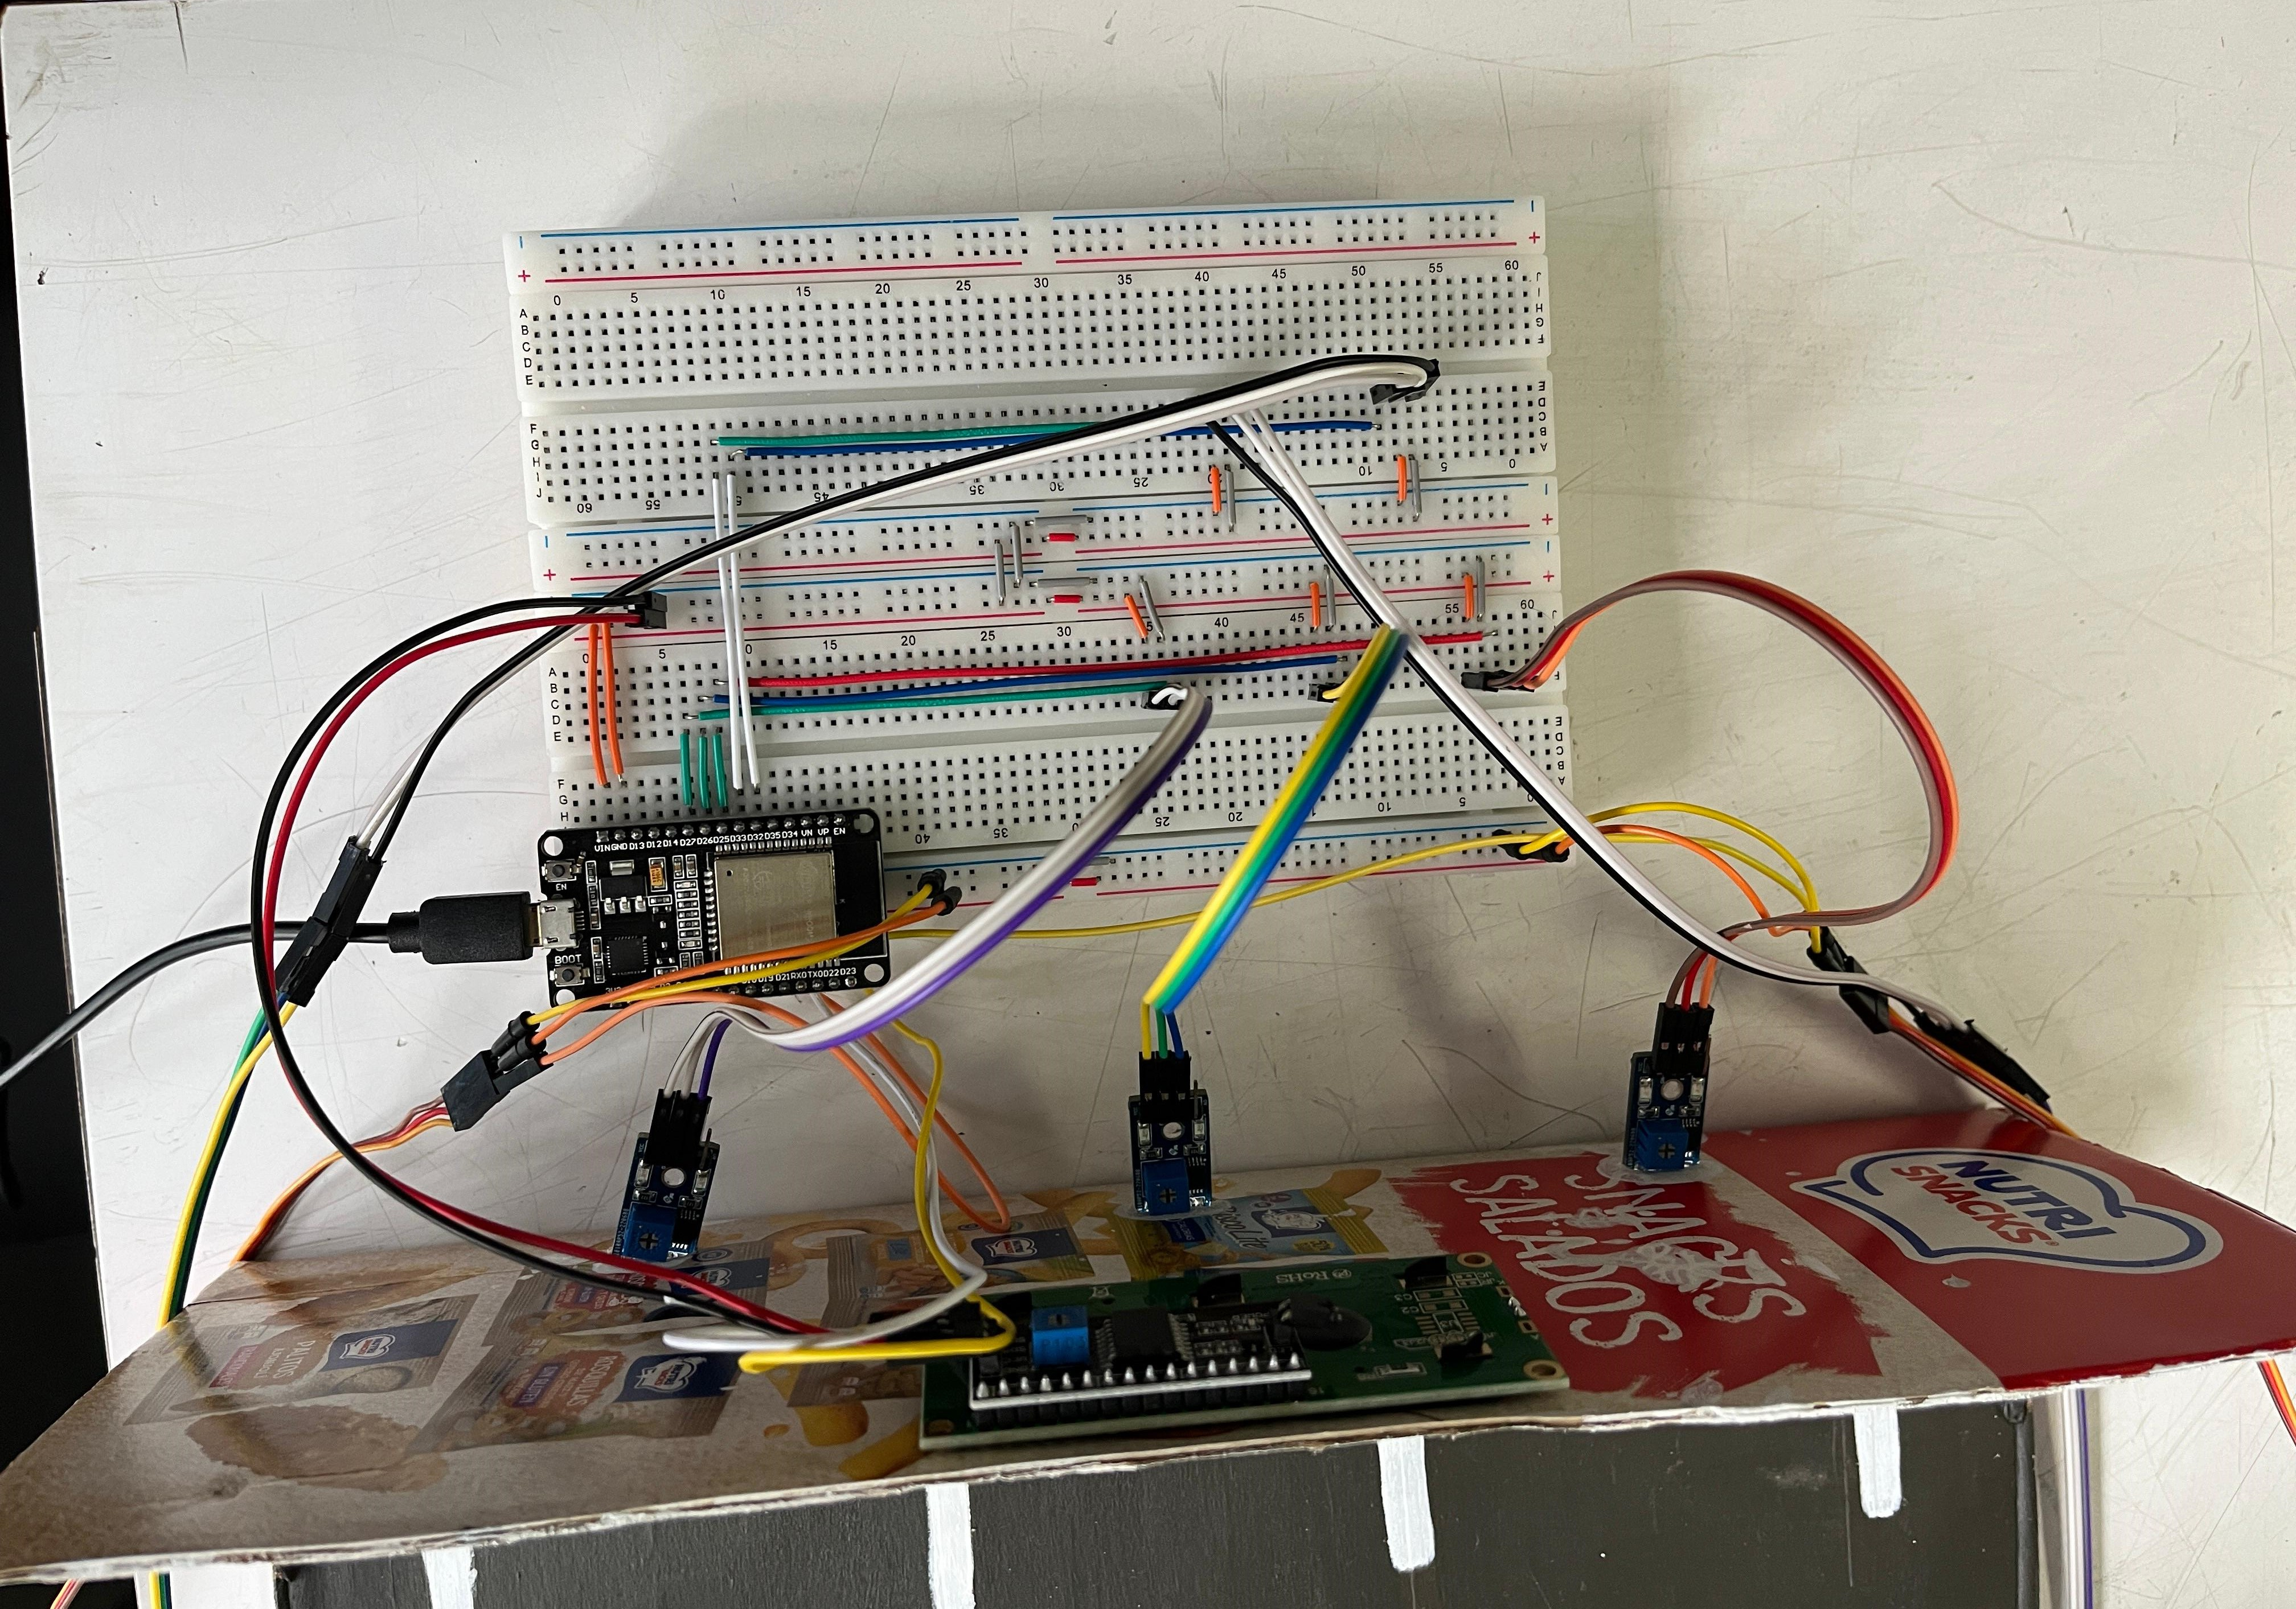
\includegraphics[width=0.7\linewidth]{Imagenes/circuito.jpg}
    \caption{Circuito para conectar la placa a una batería de 9V}
    \label{fig:5}
\end{figure}

En las figuras anteriores se puede notar que cuando se detecta un nivel de batería de 0V el led PG14 de la placa se enciende de forma parpadeante, pues se debe alertar cuando la batería se aproxima al nivel mínimo operativo del microcontrolador.

El análisis de voltaje medido se encuentra en la siguiente sección.


Asimismo, otra funcionalidad implementada es la de un botón que permite activar o desactivar las comunicaciones por medio de USART/USB. A continuación se muestra cómo al presionar el botón se cambia el estado en la pantalla a ON y comienza a parpadear la luz led PG13.

\begin{figure}[H]
    \centering
    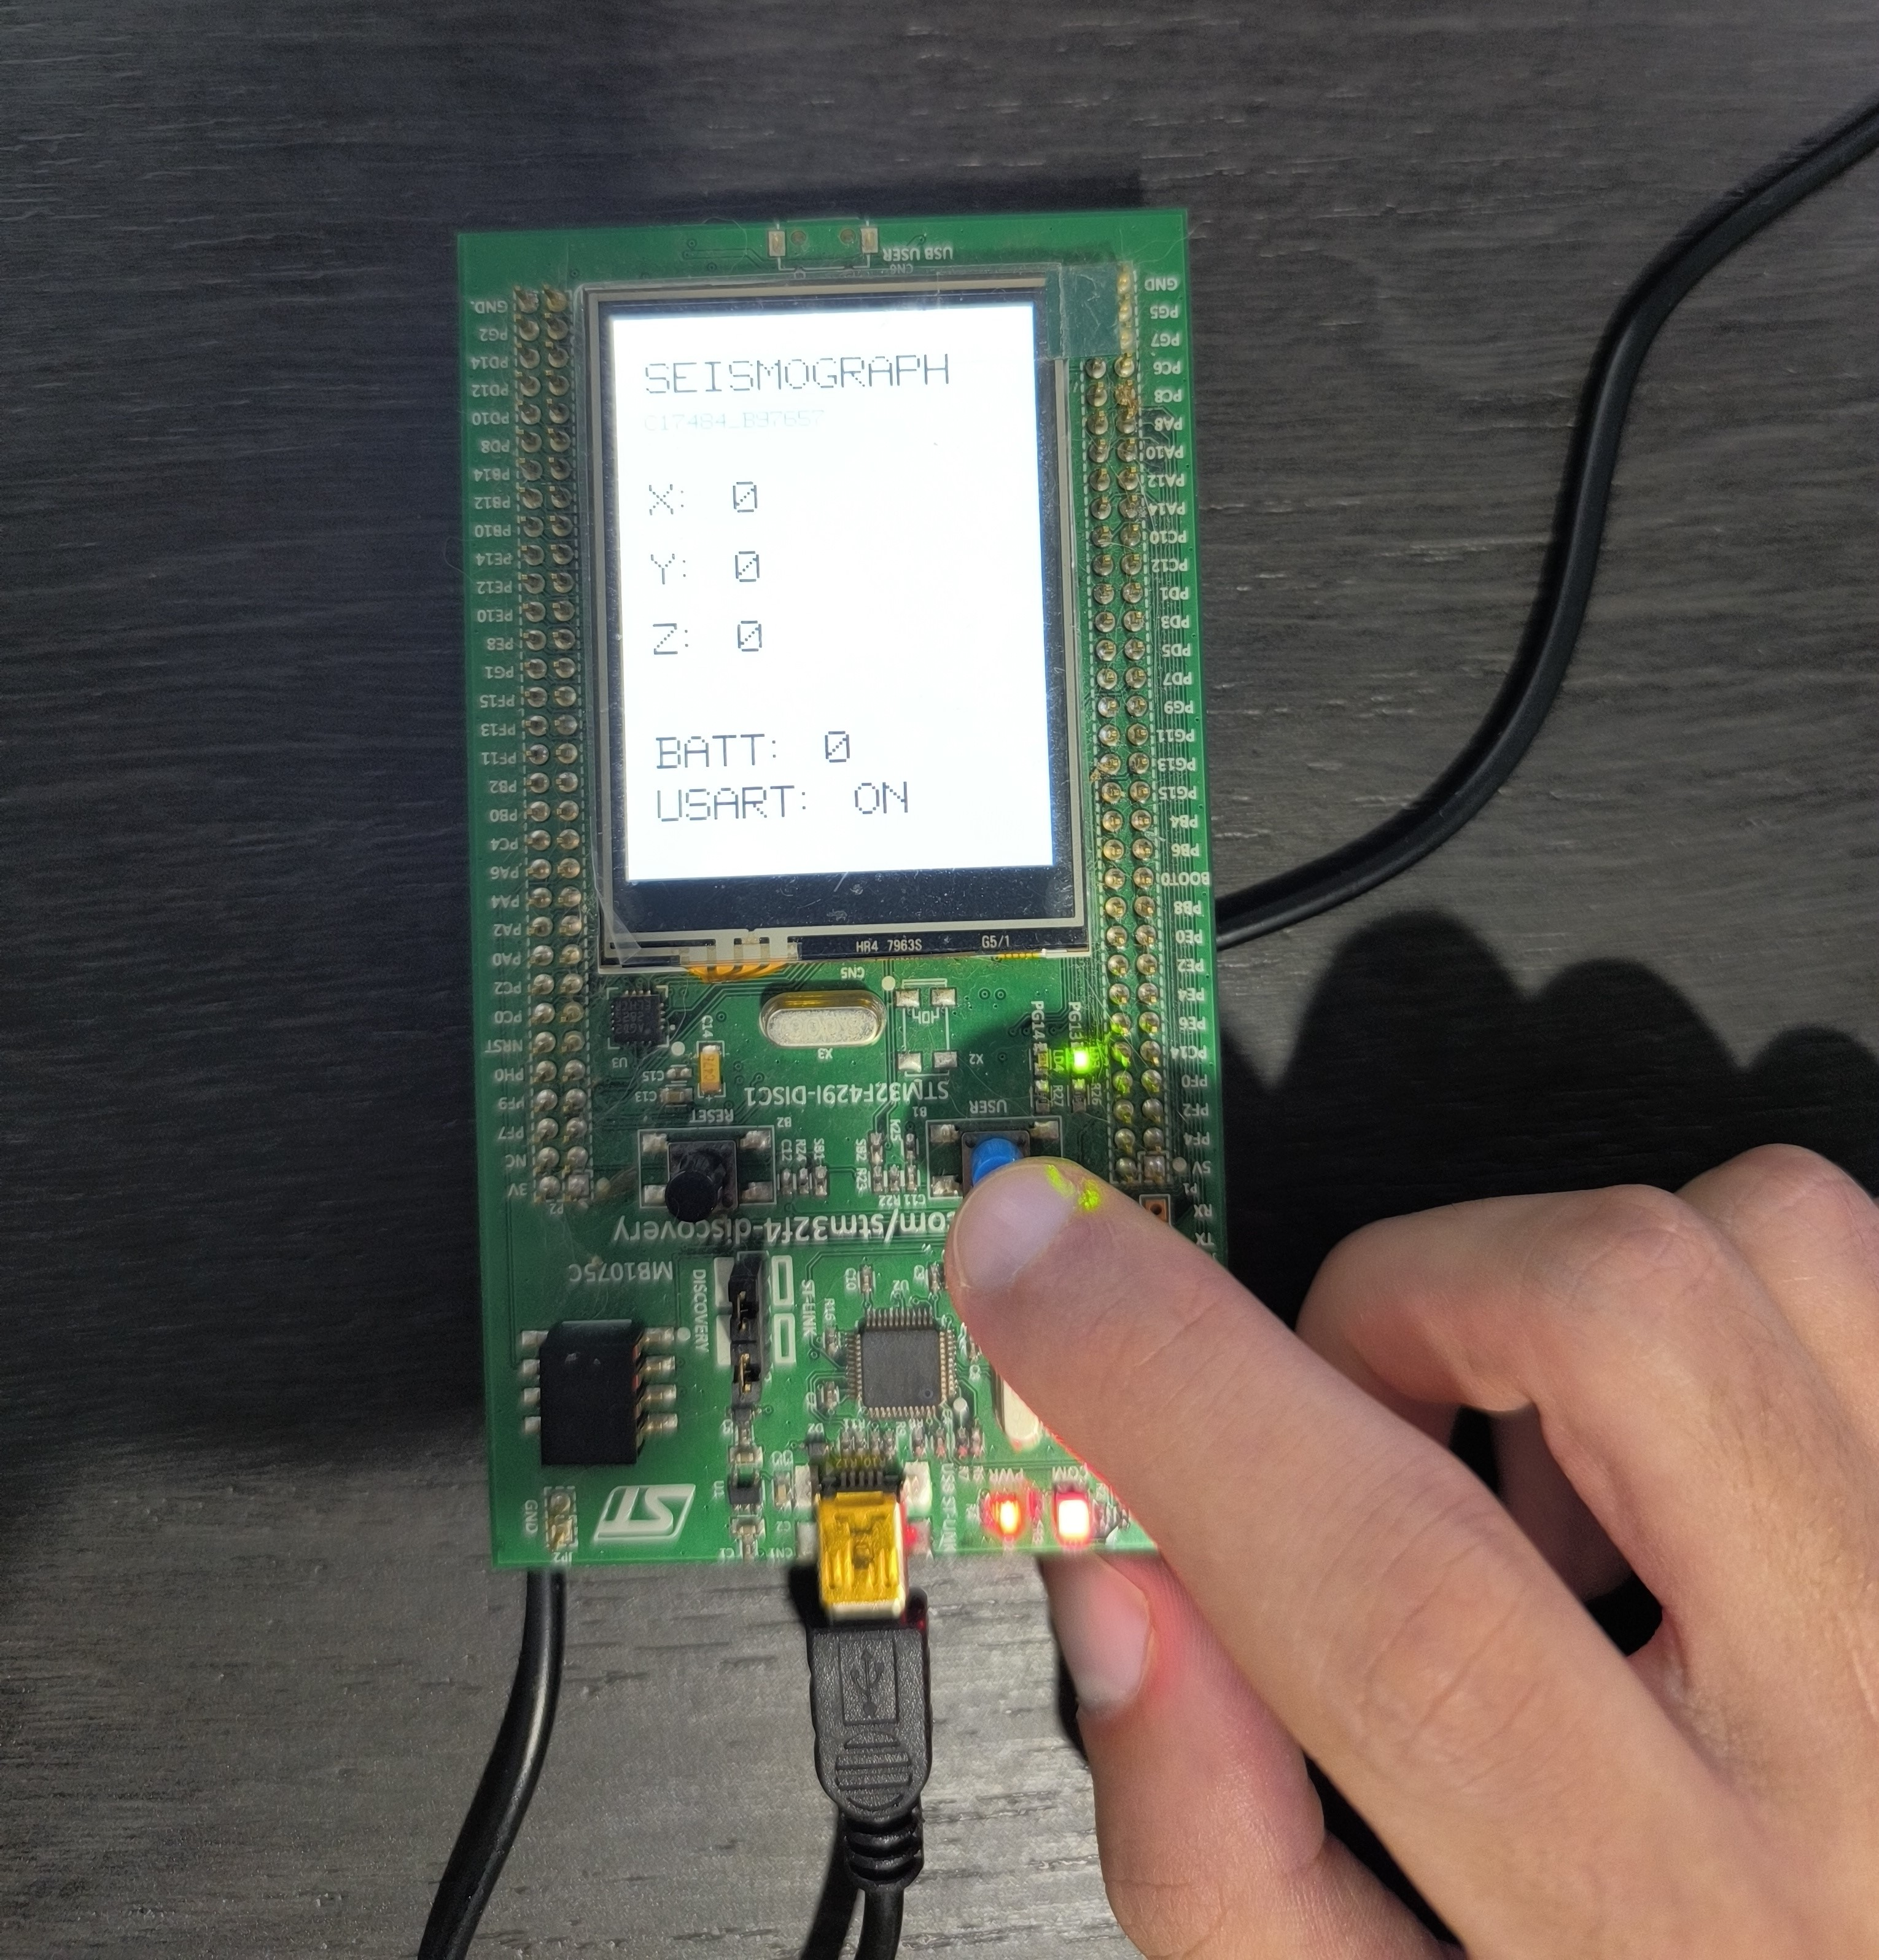
\includegraphics[width=0.5\linewidth]{Imagenes/led.jpg}
    \caption{USB COM activado}
    \label{fig:5}
\end{figure}

Finalmente, se creó un código de Python capaz de leer y escribir al puerto serial/USB y enviar la información recolectada por la placa a un dashboard de Thingsboard. Los valores que se imprimen y el dashboard de Thingsboard se pueden observar en las siguientes imágenes.
\begin{figure}[H]
    \centering
    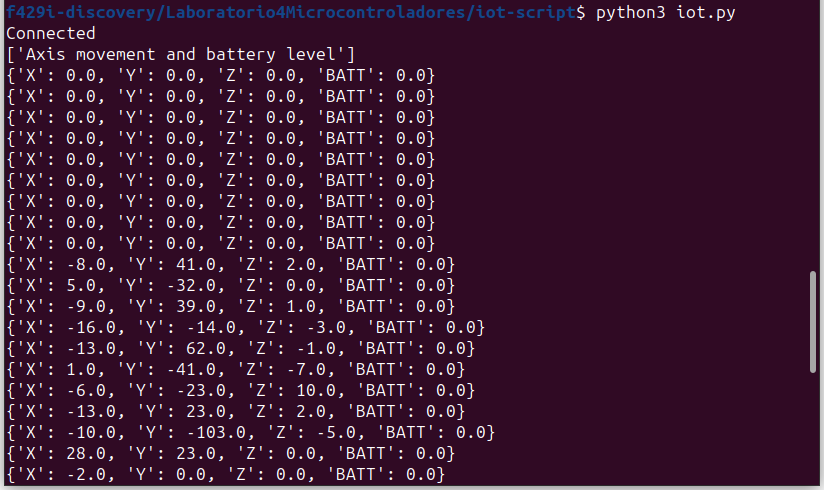
\includegraphics[width=0.8\linewidth]{Imagenes/consola.png}
    \caption{Valores enviados}
    \label{fig:5}
\end{figure}

\begin{figure}[H]
    \centering
    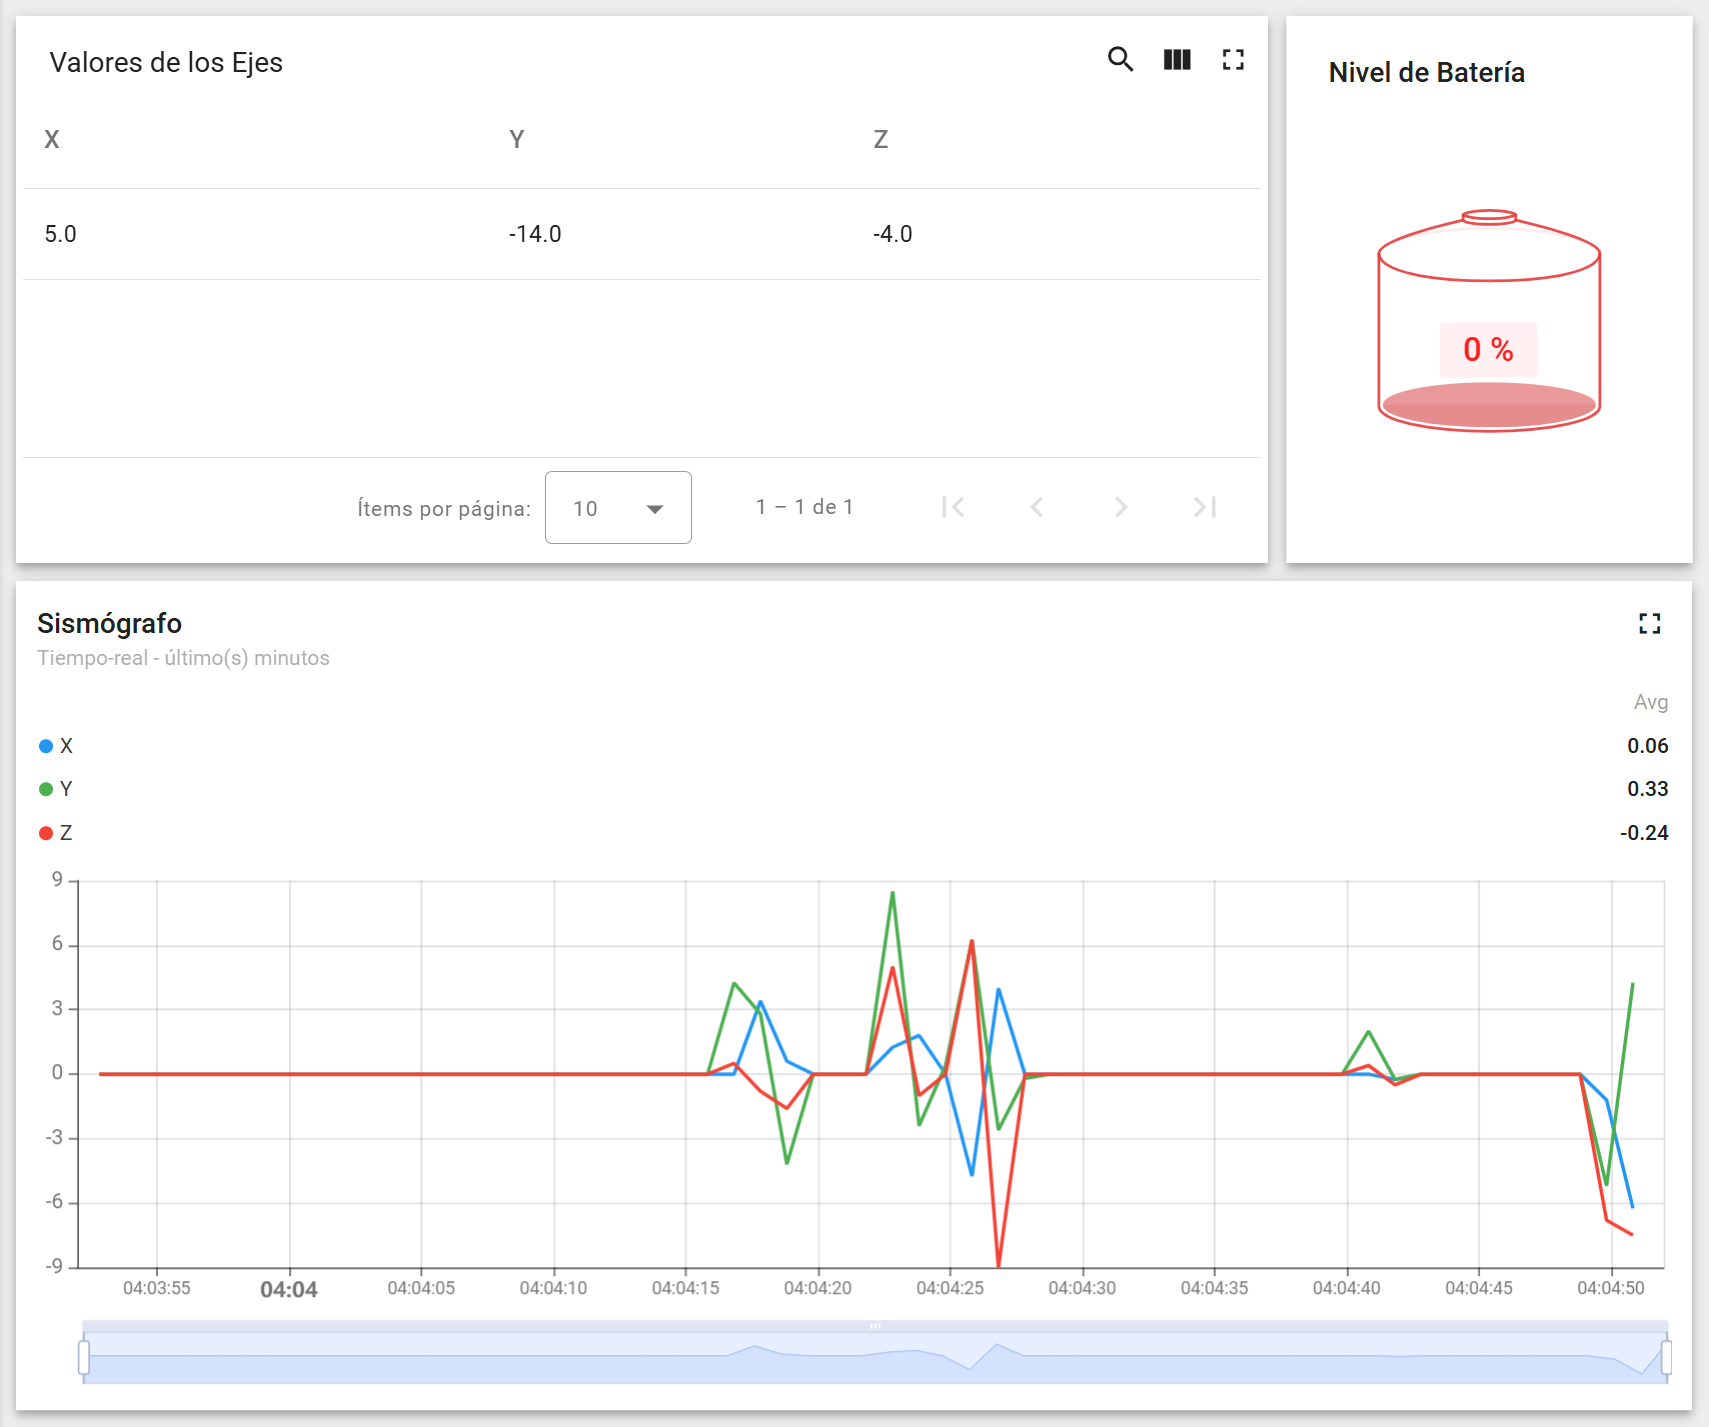
\includegraphics[width=1\linewidth]{Imagenes/dash.png}
    \caption{Dashboard de Thingsboard del Sismógrafo para varios valores medidos}
    \label{fig:5}
\end{figure}

\subsection{Análisis electrónico}

Además de los códigos utilizados para darle instrucciones al microcontrolador, se realizó un circuito para conectar este a una batería de 9V, la cual se encontraba a un nivel de 7.55V. Tal como se mencionó anteriormente, se emplearon 3 resistencias (1k $\Omega$, 220 $\Omega$ y 330 $\Omega$) para realizar un divisor de tensión y regular esta a 5V. Mediante el uso de un multímetro se midió la tensión a la salida del regulador, obteniendo los 4.87V teóricos calculados previamente.

\begin{figure}[H]
    \centering
    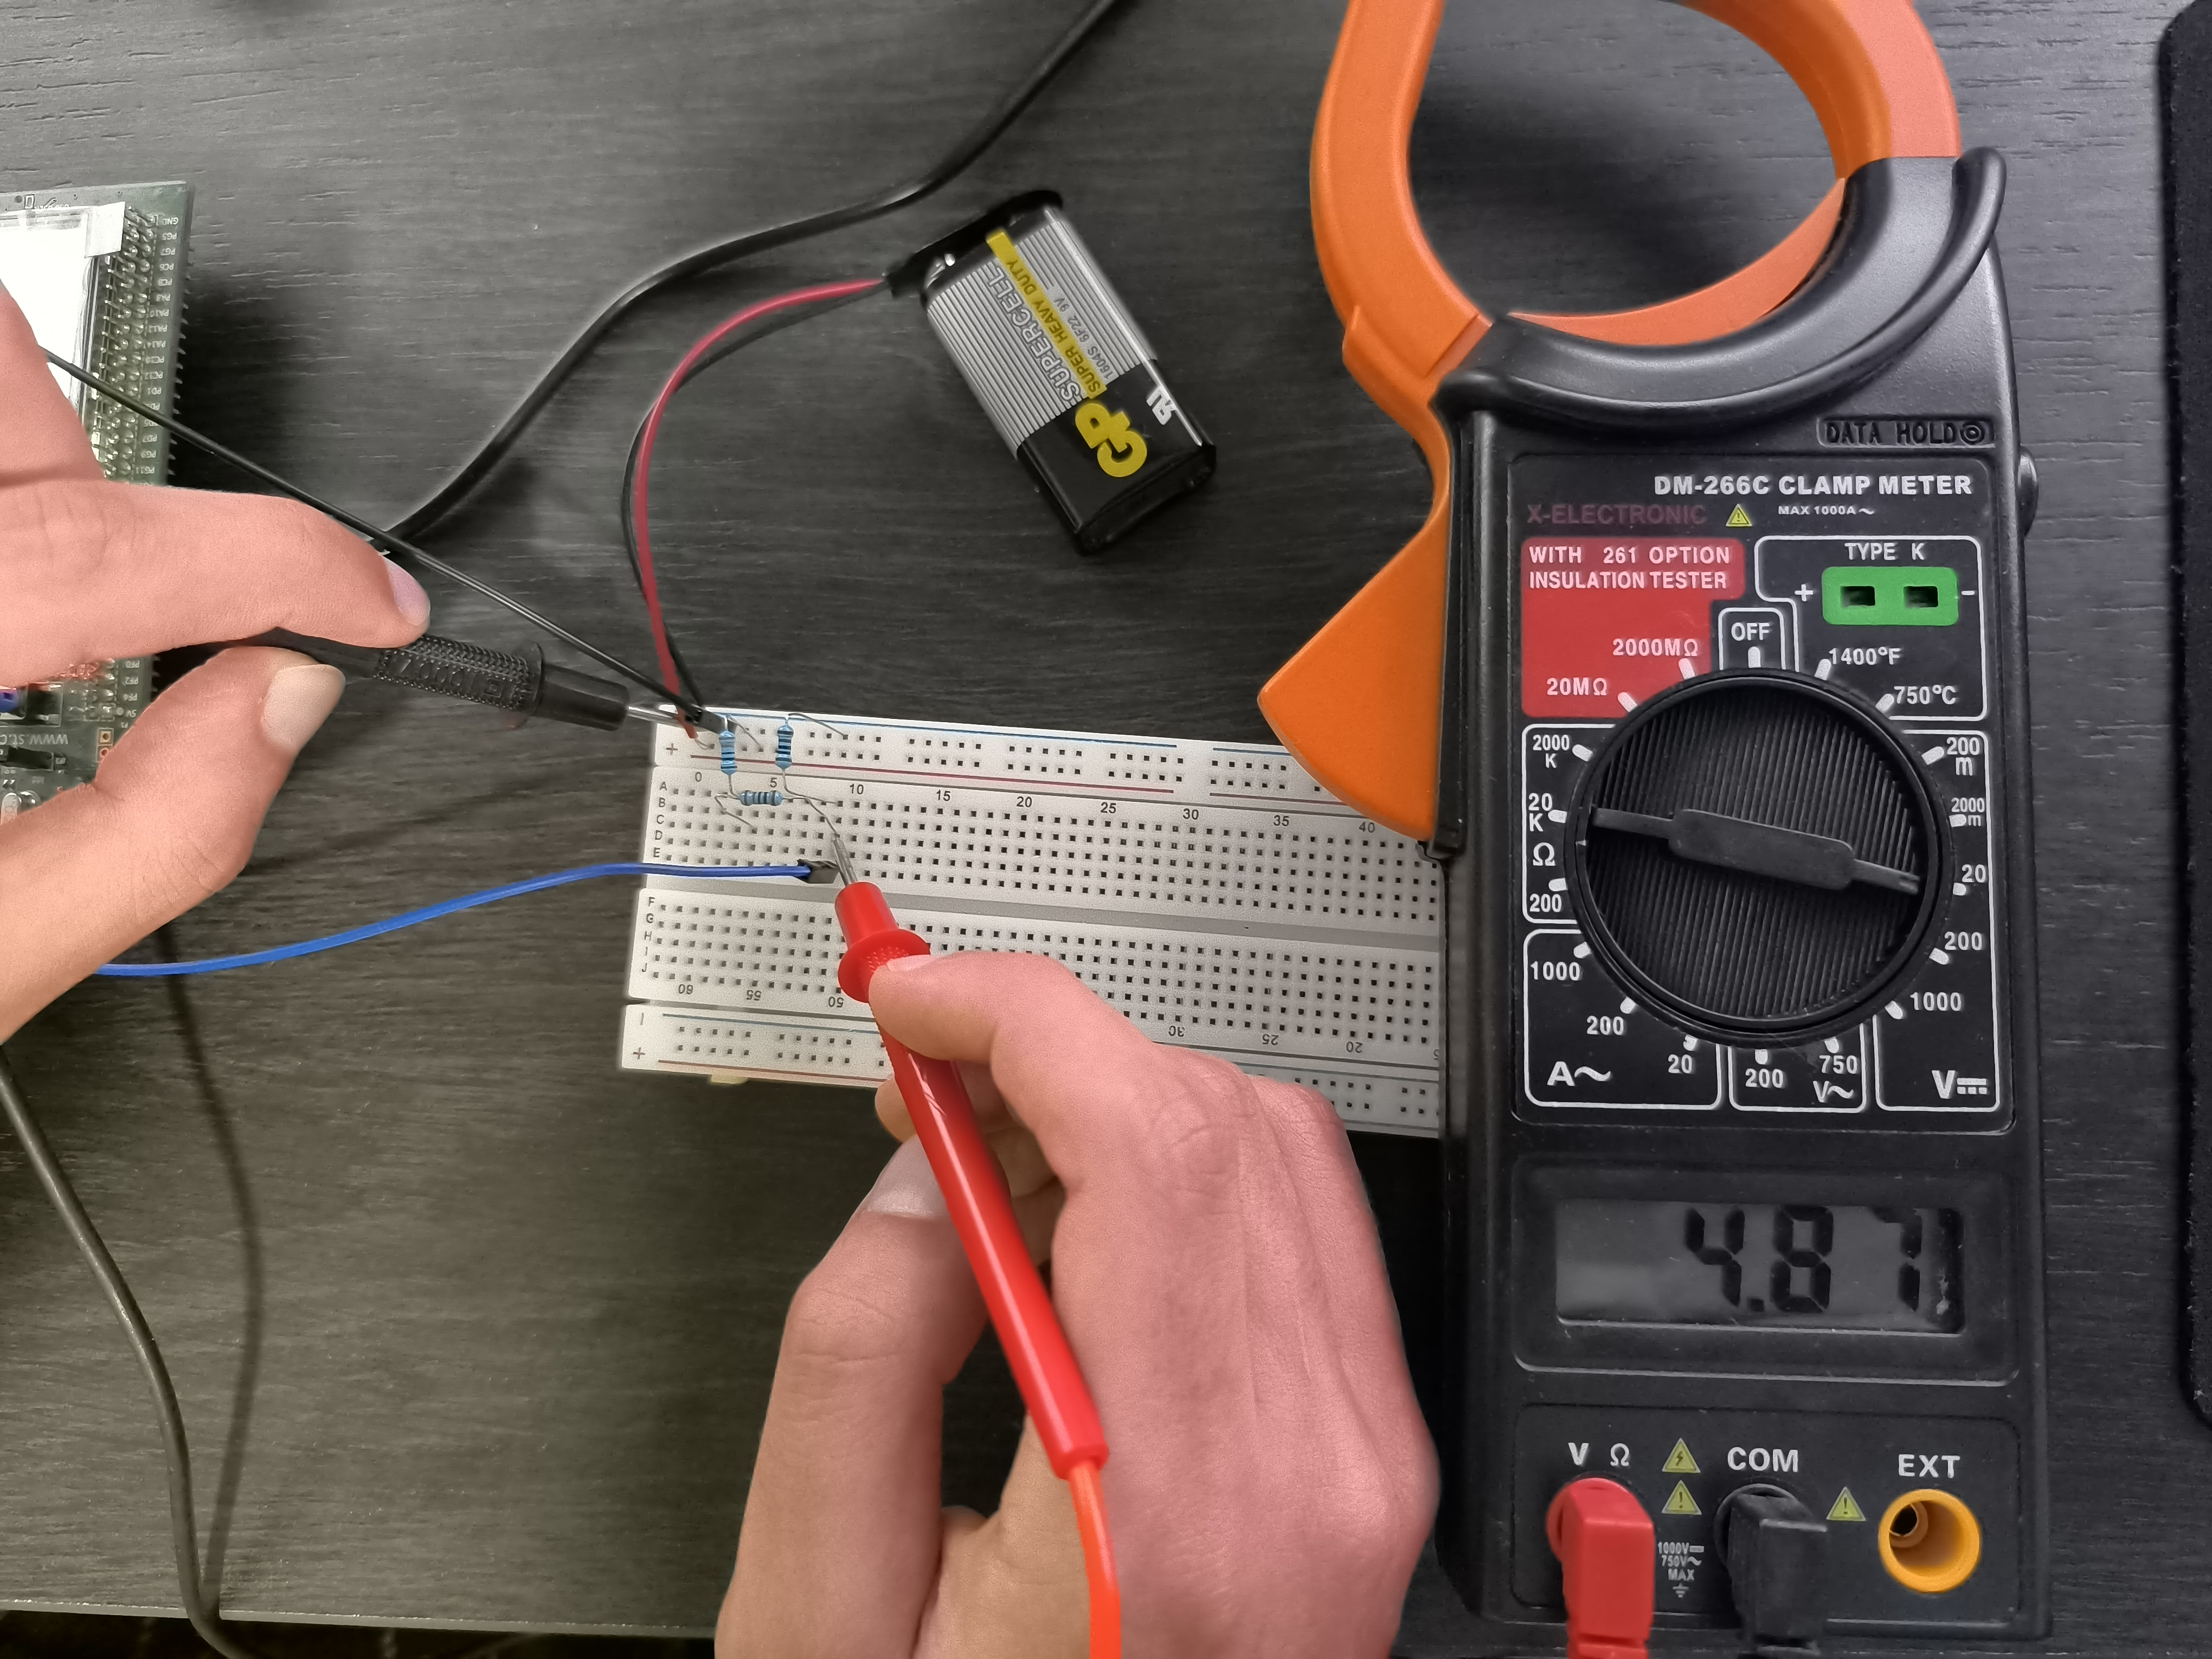
\includegraphics[width=0.83\linewidth]{Imagenes/bat.jpg}
    \caption{Valor medido a la salida del regulador}
    \label{fig:5}
\end{figure}

\begin{figure}[H]
    \centering
    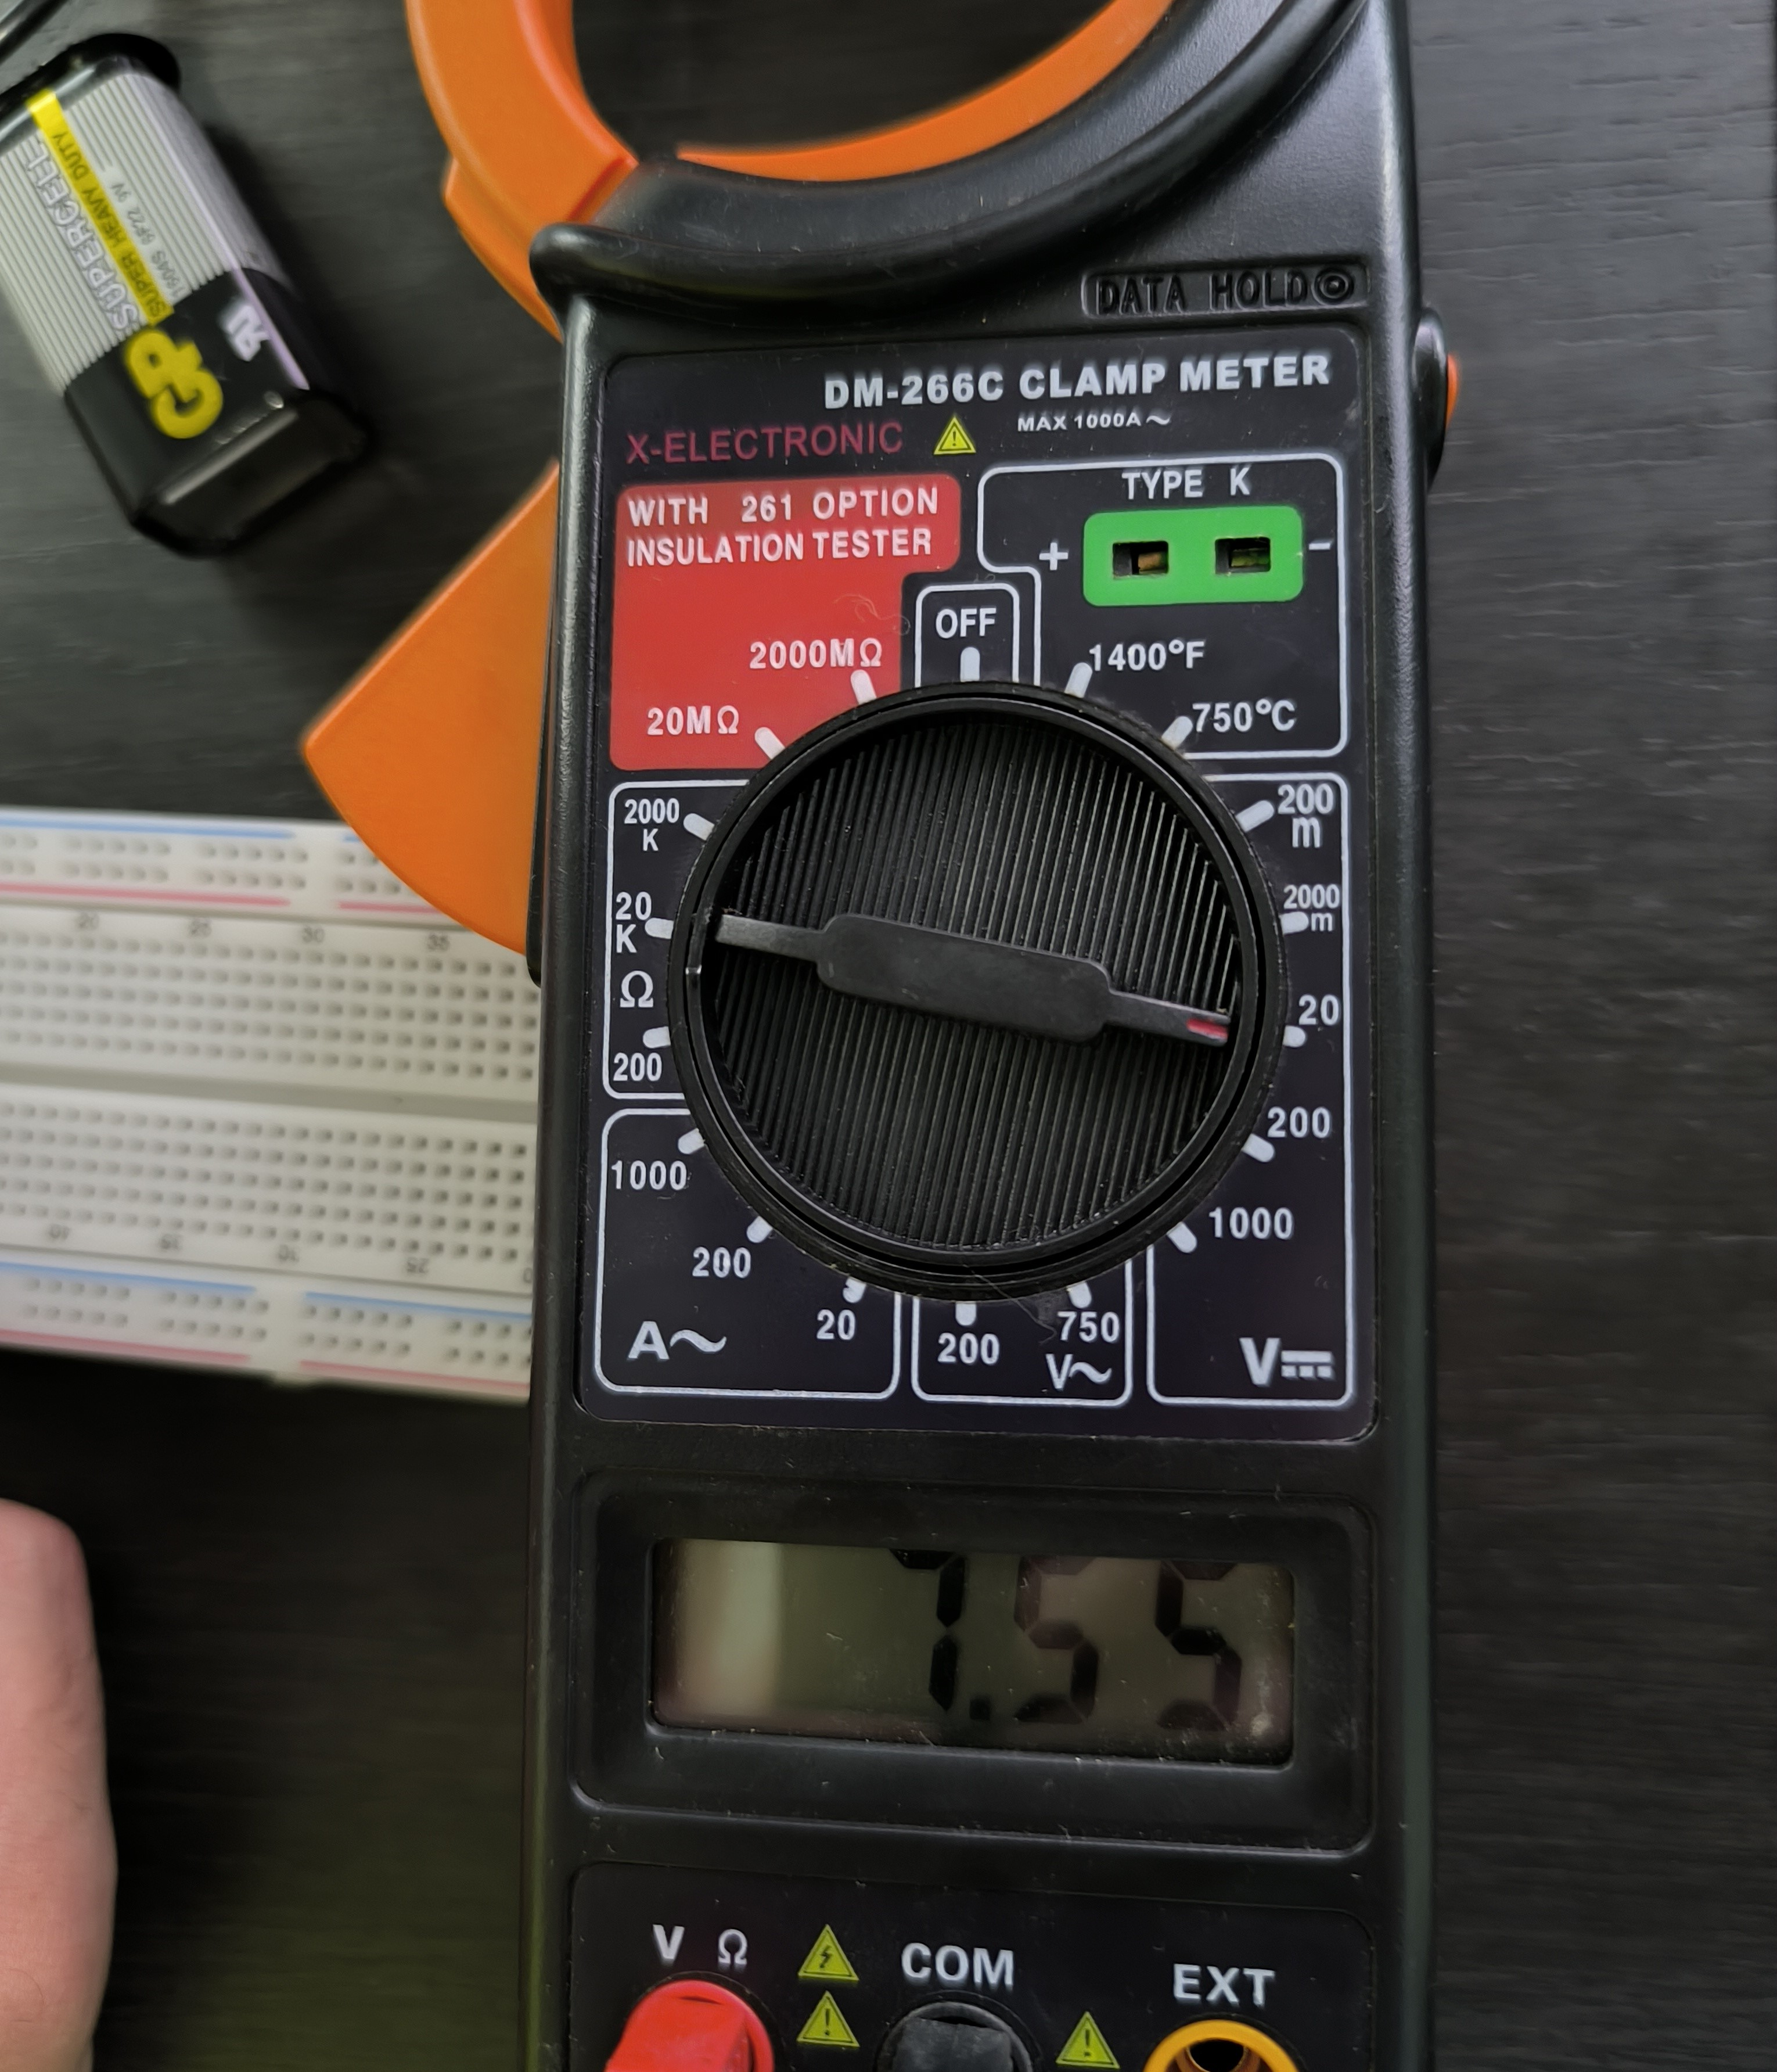
\includegraphics[width=0.6\linewidth]{Imagenes/volt.jpg}
    \caption{Tensión medida de la batería}
    \label{fig:5}
\end{figure}

Se configuró el código para leer la señal de tensión usando el pin PA3, mientras que la tierra se conectó al pin GND. Se debe resaltar que no fue posible leer el valor correcto de la tensión de la batería. Se intentaron distintas alternativas de código y con distintos pines de la placa, pero ninguna con éxito. No obstante, el circuito realizado cumple con lo requerido y las funcionalidades de impresión del valor en la LCD, el parpadeo de una led de alarma si el valor es bajo y la implementación en Thingsboard fueron efectuadas correctamente.

\section{Conclusiones y recomendaciones}

El sensor L3GD20 ha mostrado alta sensibilidad y precisión en la detección de oscilaciones, cumpliendo con los requisitos del sismógrafo para detectar vibraciones o giros. Se obtuvieron valores positivos y negativos según el movimiento de forma acertada.

La implementación de protocolos USART y SPI permitió una comunicación eficiente con periféricos como el display LCD y el sensor de movimiento, asegurando una respuesta rápida en la transmisión de datos y enviando estos al puerto serial para posteriormente ser leídos y mostrados en la plataforma IoT.

El uso de la plataforma Thingsboard permitió una visualización remota confiable de los datos del sismógrafo, facilitando el monitoreo de las mediciones en tiempo real, pues a través de widgets en el dashboard la información se procesa de una forma más accesible. Además, la correcta programación del envió de los datos hacia esta plataforma fue esencial, ya que cuenta con un formato específico.

Aunque el circuito para medir la tensión fue funcional, existieron dificultades para lograr las lecturas correspondientes del nivel de batería, lo que requiere ajustes adicionales en el código. Se recomienda revisar las configuraciones del ADC y explorar otras alternativas del código para lograr satisfactoriamente las mediciones de la batería.

Se recomienda además, iniciar explorando cada uno de los ejemplos que ofrece la biblioteca libopencm3, ya que estos ejemplos son muy útiles y cubren una amplia gama de las funcionalidades del microcontrolador STM32F429. Estos ejemplos proporcionan una base sólida para comprender tanto el uso de la biblioteca como el comportamiento y las capacidades del microcontrolador, facilitando así el aprendizaje y la experimentación. Por otro lado, es sumamente necesario iniciar con antelación este laboratorio, con el fin de conseguir los componentes necesarios a tiempo y evacuar dudas en el proceso, ya que se trata de un microcontrolador complejo.

\begin{thebibliography}{}
\bibitem{hoja}
STM Microelectronics, \textit{STM32F427xx STM32F429xx} [Online]. Disponible en:
\url{https://www.st.com/resource/en/datasheet/stm32f427vg.pdf}

\bibitem{sensor}
STMicroelectronics, \textit{L3GD20 MEMS Motion Sensor: Three-Axis Digital Output Gyroscope}, Datasheet [Online]. Disponible en: \url{https://www.st.com/resource/en/datasheet/l3gd20.pdf}.

\bibitem{gpio}
Renesas. \textit{Essentials of microcontroller use learning about peripherals: GPIO}. Disponible en: \url{https://www.renesas.com/us/en/support/engineer-school/mcu-programming-peripherals-01-gpio} .

\bibitem{electronics_tutorials}
Electronics Tutorials. \textit{Analogue to digital converter}. Disponible en: \url{https://www.electronics-tutorials.ws/combination/analogue-to-digital-converter.html}.

\bibitem{spi}
Grusin, M. \textit{Serial peripheral interface (SPI)}. Disponible en: \url{https://learn.sparkfun.com/tutorials/serial-peripheral-interface-spi/all}.

\bibitem{usart}
Texas Instruments, \textit{Universal synchronous asynchronous receive/transmit USART}. Disponible en: \url{https://www.ti.com/sc/docs/products/micro/msp430/userguid/ag_12.pdf} .

\bibitem{usb}
STMicroelectronics. \textit{Introduction to USB with STM32}.  Disponible en: \url{https://wiki.st.com/stm32mcu/wiki/Introduction_to_USB_with_STM32}.


\bibitem{iot}
Gillis, A. \textit{Internet of Things (IoT)}. Disponible en: \url{https://www.techtarget.com/iotagenda/definition/Internet-of-Things-IoT}.

\bibitem{libopencm3}
Libopencm3 contributors, ``libopencm3-examples,'' Disponible en: \url{https://github.com/libopencm3/libopencm3-examples}.






\end{thebibliography}





\section{Apéndices}

\includepdf[pages={5-9}]{Documentos/STM32}
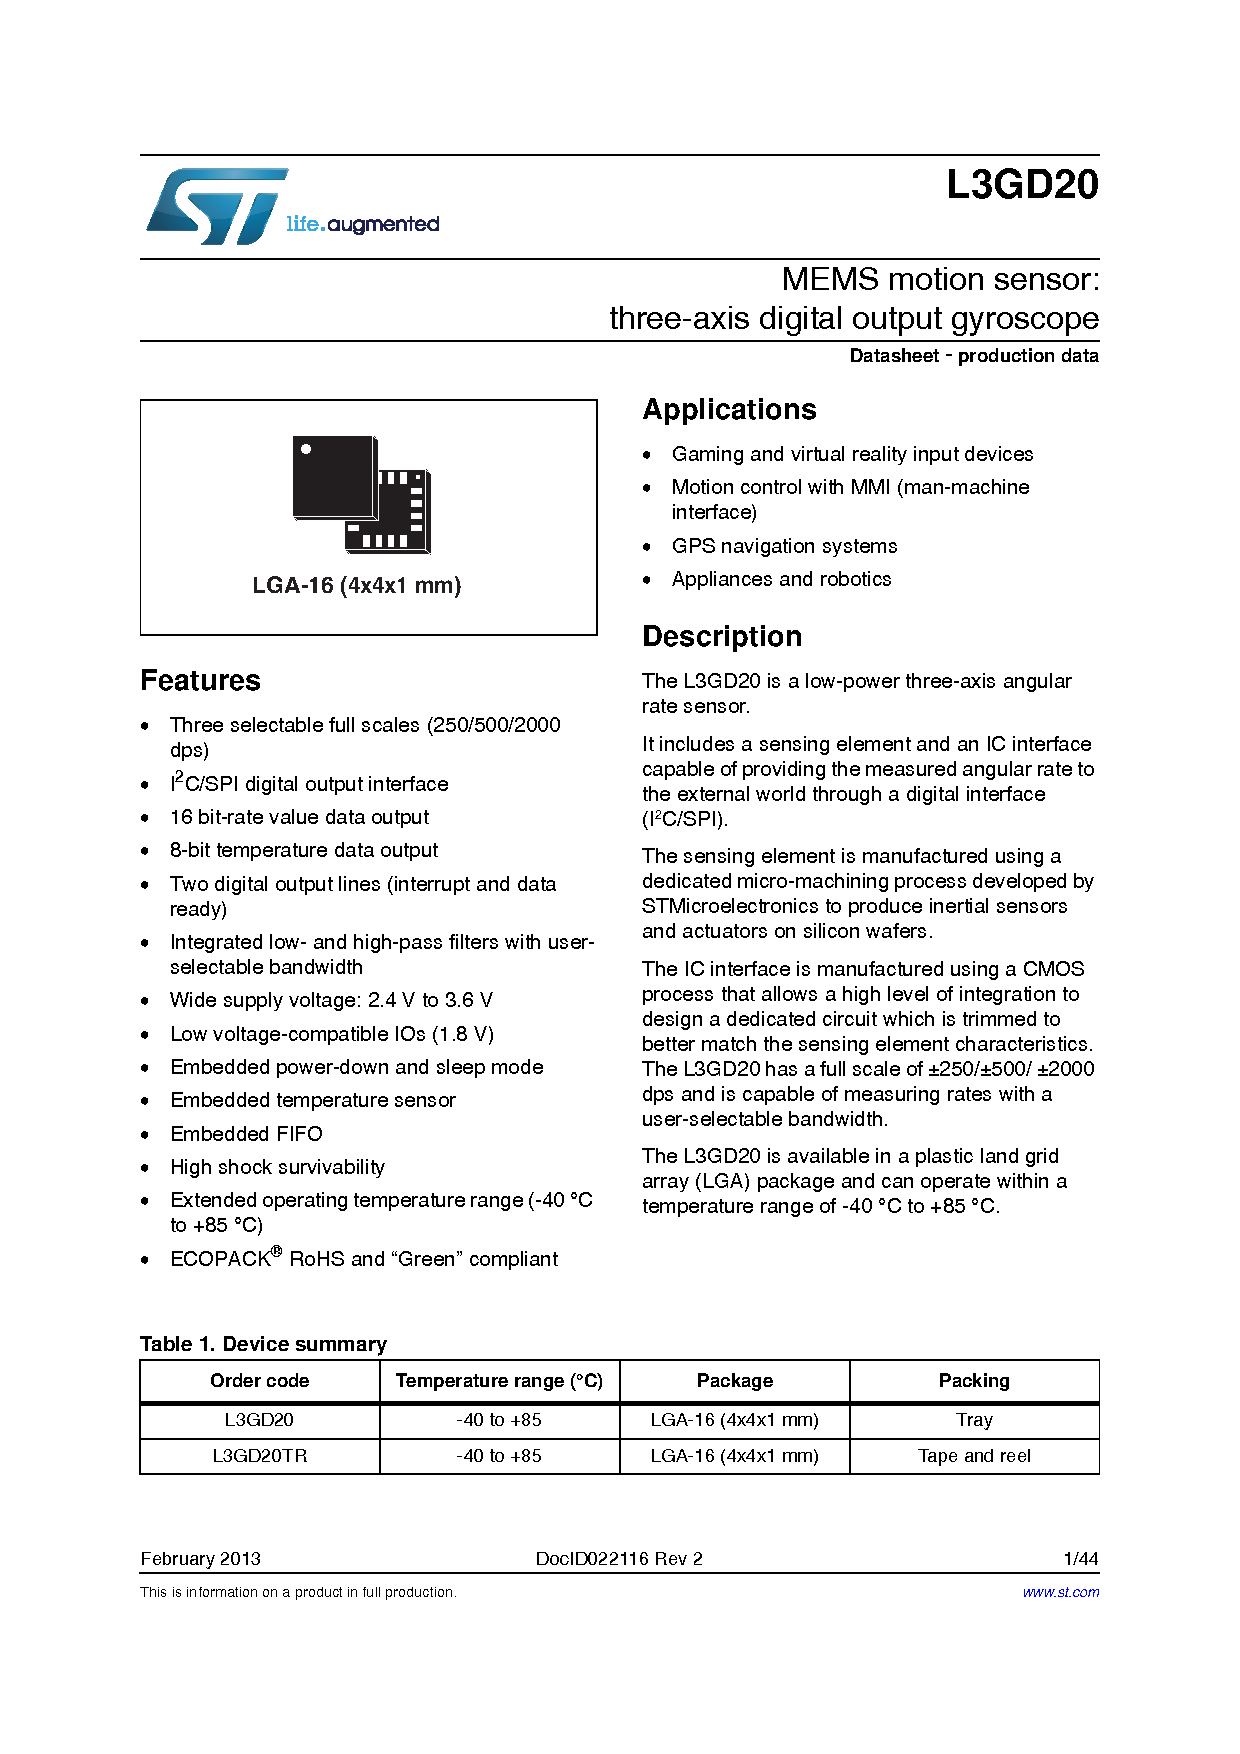
\includepdf[pages={1,7-11}]{Documentos/l3gd20}

\end{document}
